\documentclass[11pt]{beamer}

\usetheme{epfl}
\usepackage{tikz}
\usetikzlibrary{positioning,arrows.meta}
\usetikzlibrary{calc,patterns,angles,quotes, fadings}
\usetikzlibrary{decorations,fit}

\usepackage{media9}
\usepackage{amsmath}
\usepackage[thicklines]{cancel}
\usepackage{svg}
\newcommand{\citeapa}[1]{ {\tiny#1\par} }
%\usepackage{utf8}
%\usepackage{fontspec}

% primary colors
\definecolor{tumblue}{RGB}{0,101,189} % Pantone 300
\definecolor{tumorange}{RGB}{227,114,34} % Pantone 158 - Orange
\setbeamercovered{transparent}

\begin{document}
	
	\title{Data-Driven Vegetation Modeling and Tackling Representation Shift}
	\subtitle{with Few-Shot Meta-Learning Methods}
	\author{Marc Russwurm}
	\labname{EPFL-ECEO}
	\date{\today}
	
	\logofilename{epfl/epfl_red.png}
	\titlepageimage{epfl/lacleman}
	\event{Deep Learning for Environment}
	\presentation{Representation Shift and Few-Shot Meta-Learning Methods}
	\speaker{Marc Russwurm}
	
	\begin{frame}[plain]
		\maketitle
	\end{frame}

	\begin{frame}{Structure}
		
		\begin{enumerate}
			\item Data-Driven Vegetation Modeling and 
			\begin{itemize}
				\item why is it meaningful
				\item data-driven verus model-driven approaches
			\end{itemize}
			\item<2-> Tackling Representation Shift 
			\begin{itemize}
				\item when does it arise?
				\item regional representations
			\end{itemize}
			\item<3> with Few-Shot Meta-Learning Methods
			\begin{itemize}
				\item seeing our remote sensing data as a dataset-of-datasets
				\item Model-agnostic meta-learning as one algorithm to tackle it.
			\end{itemize}
		\end{enumerate}
		
	\end{frame}

	\begin{frame}{Vegetation Modeling}
		\begin{tikzpicture}
			\node[fill=EPFLred, inner sep=1em, text=white, font=\bfseries]{Vegetation Modeling};
		\end{tikzpicture}
	\end{frame}


	\begin{frame}
		\frametitle{Why do we want to classify vegetation?}
		\begin{columns}
			\column{.5\textwidth}
			{\scriptsize
			\begin{description}
				\item[Zero Hunger] estimating the \textbf{crop yield} \& predict \textbf{food prices}, shortages.
				\item<2->[Climate Action] by monitoring \textbf{vegetation changes} over time (desertification).
				\item<3->[Life on Land] human life depends on \textbf{agriculture}, animal life on \textbf{biotopes}.
				%				\item Precision agriculture: sd
			\end{description}
			}
			\column{.5\textwidth}
			
\includegraphics[width=\textwidth]{images/sdg_goals.pdf}
		\end{columns}
		
	\end{frame}

	\begin{frame}{Remote Sensing Data in Abundance}
		\begin{columns}[t]
			\column{.33\textwidth}
				MODIS
				\includemedia[
				width=\textwidth,
				activate=pageopen,
				addresource=mp4/apenne_modis_ndvi.mp4,
				flashvars={source=mp4/apenne_modis_ndvi.mp4&loop=true&
					autoPlay=true}
				]{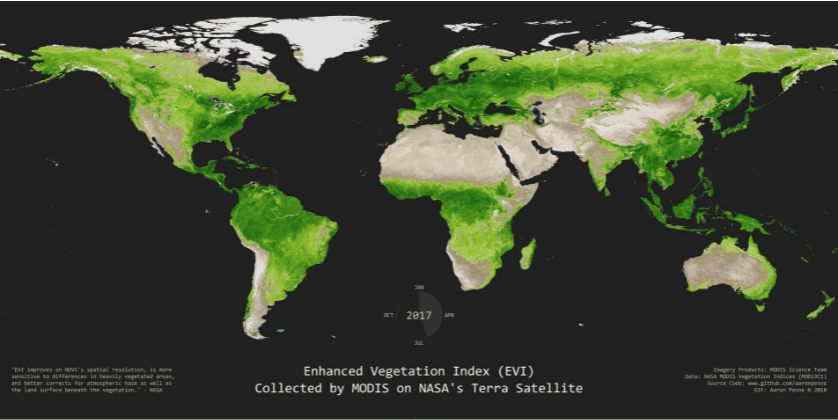
\includegraphics[width=\textwidth]{mp4/apenne_modis_ndvi.png}}{mp4/apenne_modis_ndvi.mp4}
				{\tiny visualization \href{https://github.com/aaronpenne}{Aaron Penne Github}}
			
%				\vfill
%				\scriptsize daily, global scale, 36 bands (1km by 1km pixels)
			\column{.33\textwidth}
				Sentinel/Landsat
				\includemedia[
				width=\textwidth,
				activate=pageopen,
				addresource=mp4/sentinel2.mp4,
				flashvars={source=mp4/sentinel2.mp4&loop=true&
					autoPlay=true}
				]{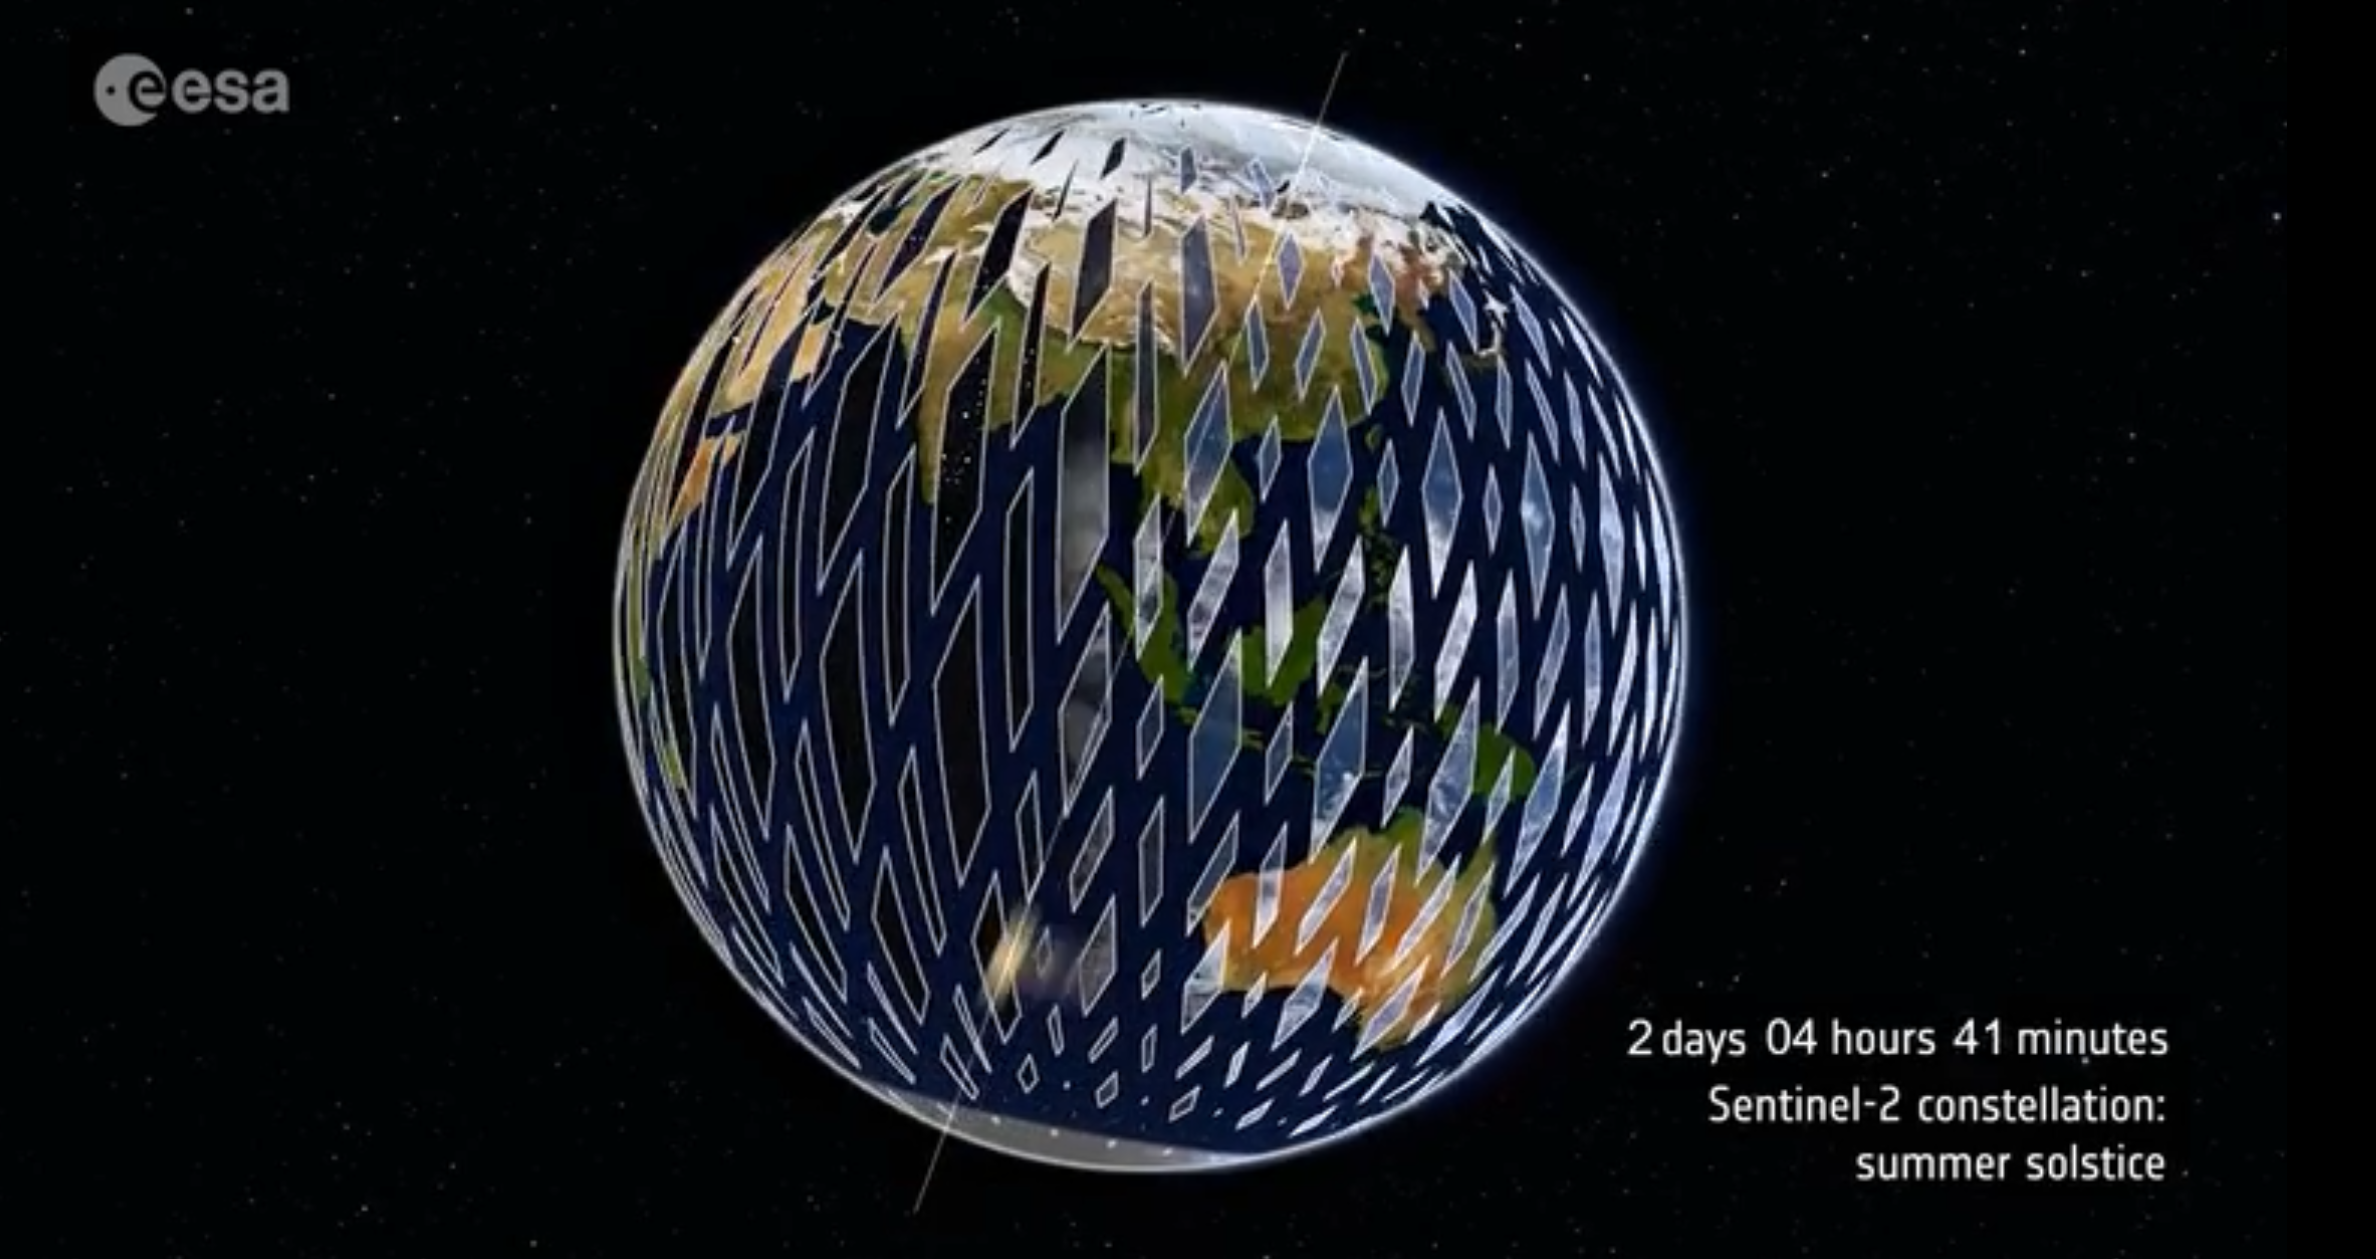
\includegraphics[width=\textwidth]{mp4/sentinel2.png}}{mp4/sentinel2.mp4}
				{\tiny visualization ESA}
%				\vfill
%				\scriptsize 2-5 days, regional scale, 13 bands (10m by 10m pixels)
			\column{.33\textwidth}
				PlanetScope
				\includemedia[
				width=\textwidth,
				activate=pageopen,
				addresource=mp4/planet_denethor.mp4,
				flashvars={source=mp4/planet_denethor.mp4&loop=true&
					autoPlay=true}
				]{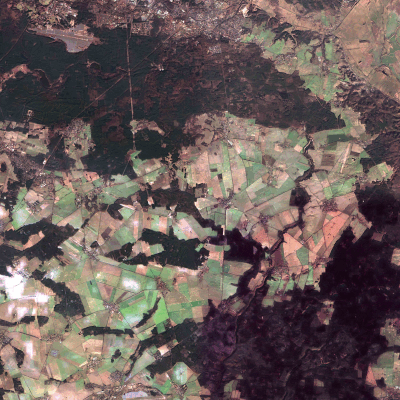
\includegraphics[width=\textwidth]{mp4/planet_denethor.png}}{mp4/planet_denethor.mp4}
				{\tiny DENETHOR dataset /\\ Kondmann et al., (2021)\par}
%				\vfill
%				\scriptsize daily, local scale, 4 bands (3m by 3m pixels)
		\end{columns}
	
		\vspace{1em}
		\small
	
		\begin{columns}
			\column{.33\textwidth}		
			\begin{itemize}
				\item daily/half-monthly
				\item 250m by 250m px
				\item 39 bands
			\end{itemize}	
			\column{.33\textwidth}
			\begin{itemize}
				\item 2-5 days
				\item 10m by 10m px
				\item 13 bands
			\end{itemize}
			\column{.33\textwidth}
			\begin{itemize}
				\item daily
				\item 3m by 3m pixels
				\item 4 bands
			\end{itemize}

	\end{columns}
	
		\vspace{3mm}
		\citeapa{Kondmann, et al., "DENETHOR: The DynamicEarthNET dataset for Harmonized, inter-Operable, analysis-Ready, daily crop monitoring from space.". NeurIPS Data Track (2021).}
	\end{frame}

	
	\begin{frame}
		\frametitle{Photosynthesis: Light $\rightarrow$ Life}
		%		\framesubtitle{Vegetation}
		
		\begin{columns}[b]
			
			\column{.5\textwidth}
			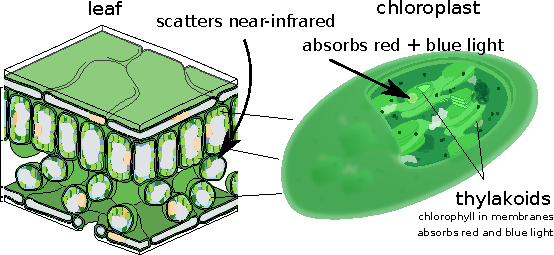
\includegraphics[width=\textwidth]{images/leaf_smallannot.pdf}
%			common remote sensing feature: $\text{NDVI} = \frac{\text{NIR} - \text{RED}}{\text{NIR} + \text{RED}}$ \\
			{\tiny Image adapted from wikipedia cc}
			%
			\column{.5\textwidth}
			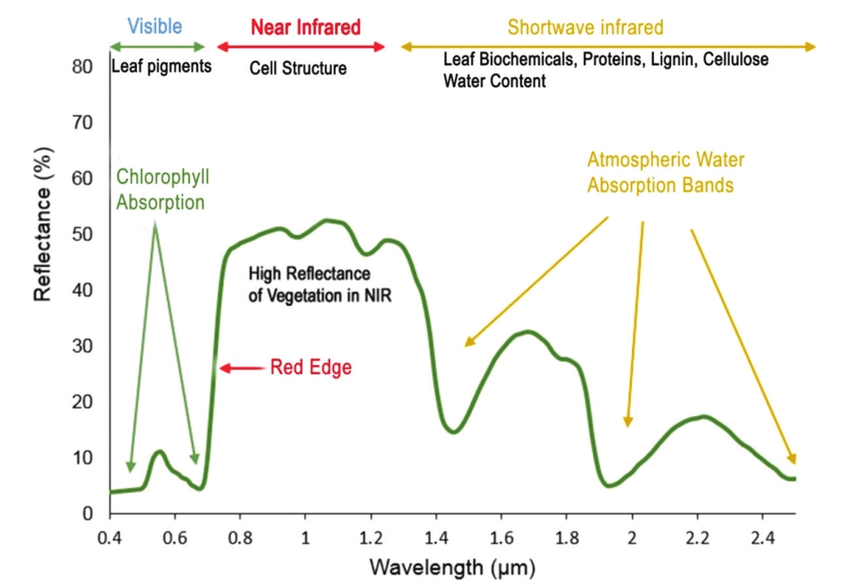
\includegraphics[width=\textwidth]{images/reflectance_vegetation}
			\tiny Image from Roman et al., (2016)
		\end{columns}
		
		\normalsize
		
		\vspace{1em}
		Normalized Difference Vegetation Index.
		\vspace{1em}
		\begin{align}
			\text{NDVI}(\text{red}, \text{nir}) = \frac{\text{nir}-\text{red}}{\text{nir}+\text{red}}
		\end{align}
		
		\vfill
		
		\citeapa{Roman, A., \& Ursu, T. (2016). Multispectral satellite imagery and airborne laser scanning techniques for the detection of archaeological vegetation marks. Landsc. Archaeol. North. Front. Rom. Emp. Porolissum, 141-152.}
		
	\end{frame}

	\begin{frame}<presentation:1>
		\frametitle{Satellite Time Series}
		
		\begin{tikzpicture}[node distance=0em]
		\node(a) at (0,0){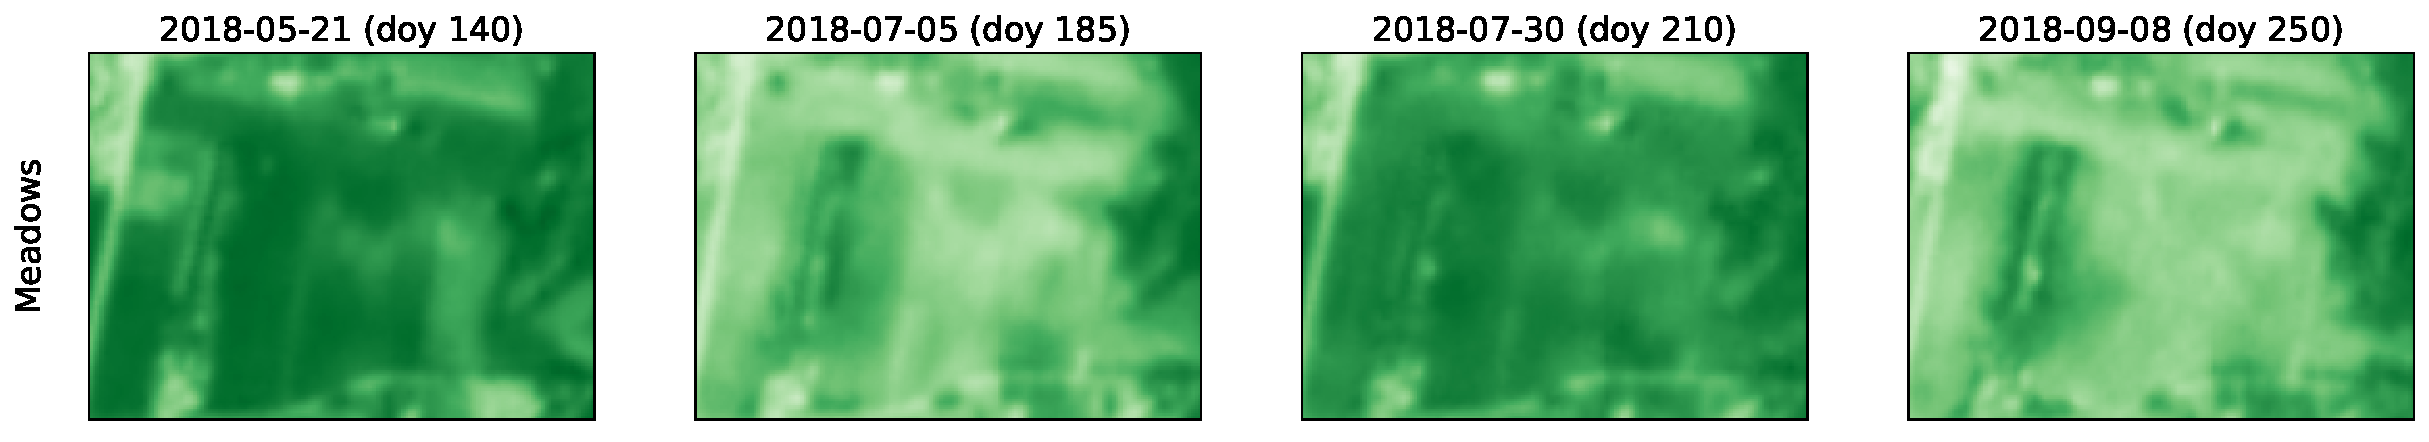
\includegraphics[width=10cm]{images/denethor/43647_Meadows_images}};
		\node(b)[below=0em of a]{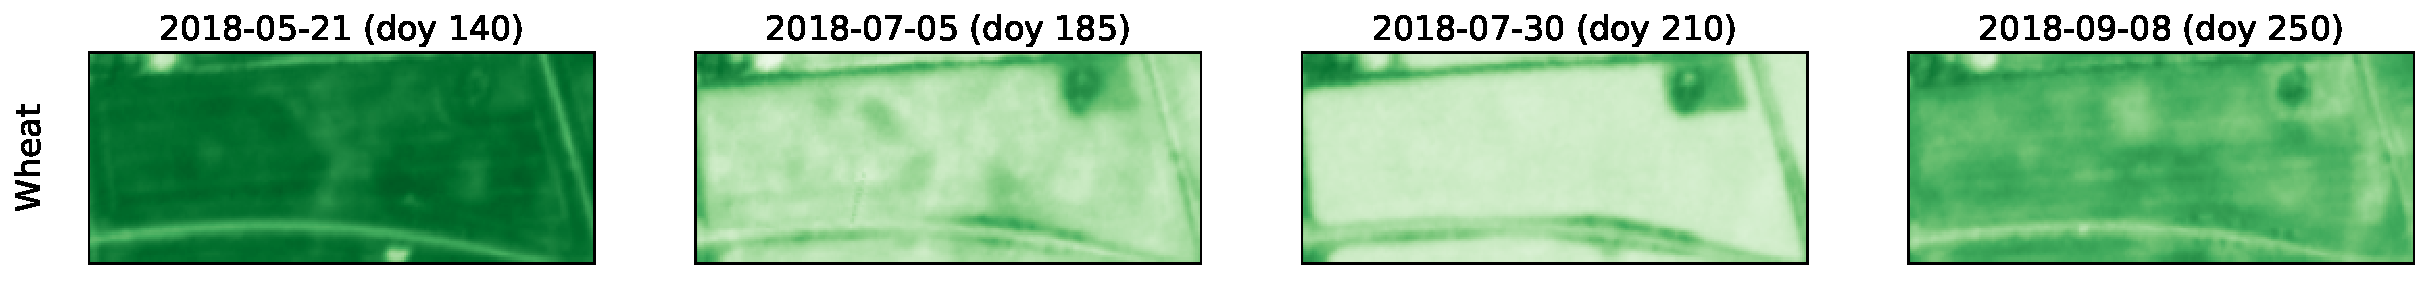
\includegraphics[width=10cm]{images/denethor/82235_Wheat_images}};
		\visible<1>{
			\node(c)[below=1cm of b, xshift=-4em]{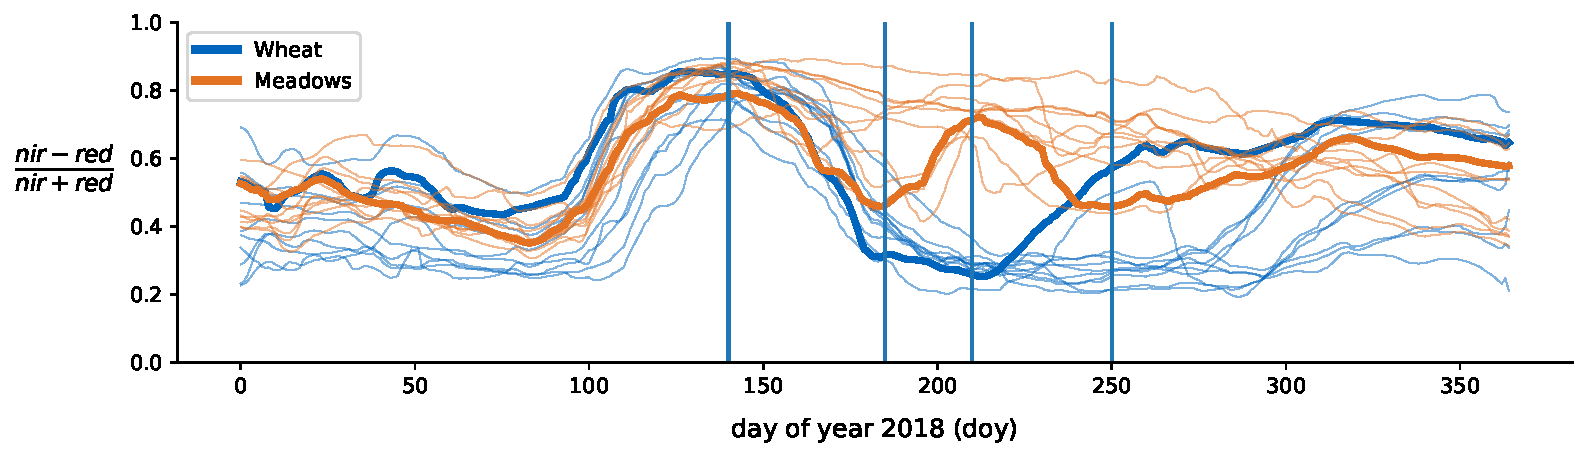
\includegraphics[width=.8\textwidth]{images/denethor/plots_2018.pdf}};
		}
	
		\visible<2>{
			\node(c)[below=1cm of b, xshift=-4em]{\includegraphics[width=.8\textwidth]{images/denethor/plotss2.pdf}};
		}
		\node(d)[right=-2em of c, yshift=1em]{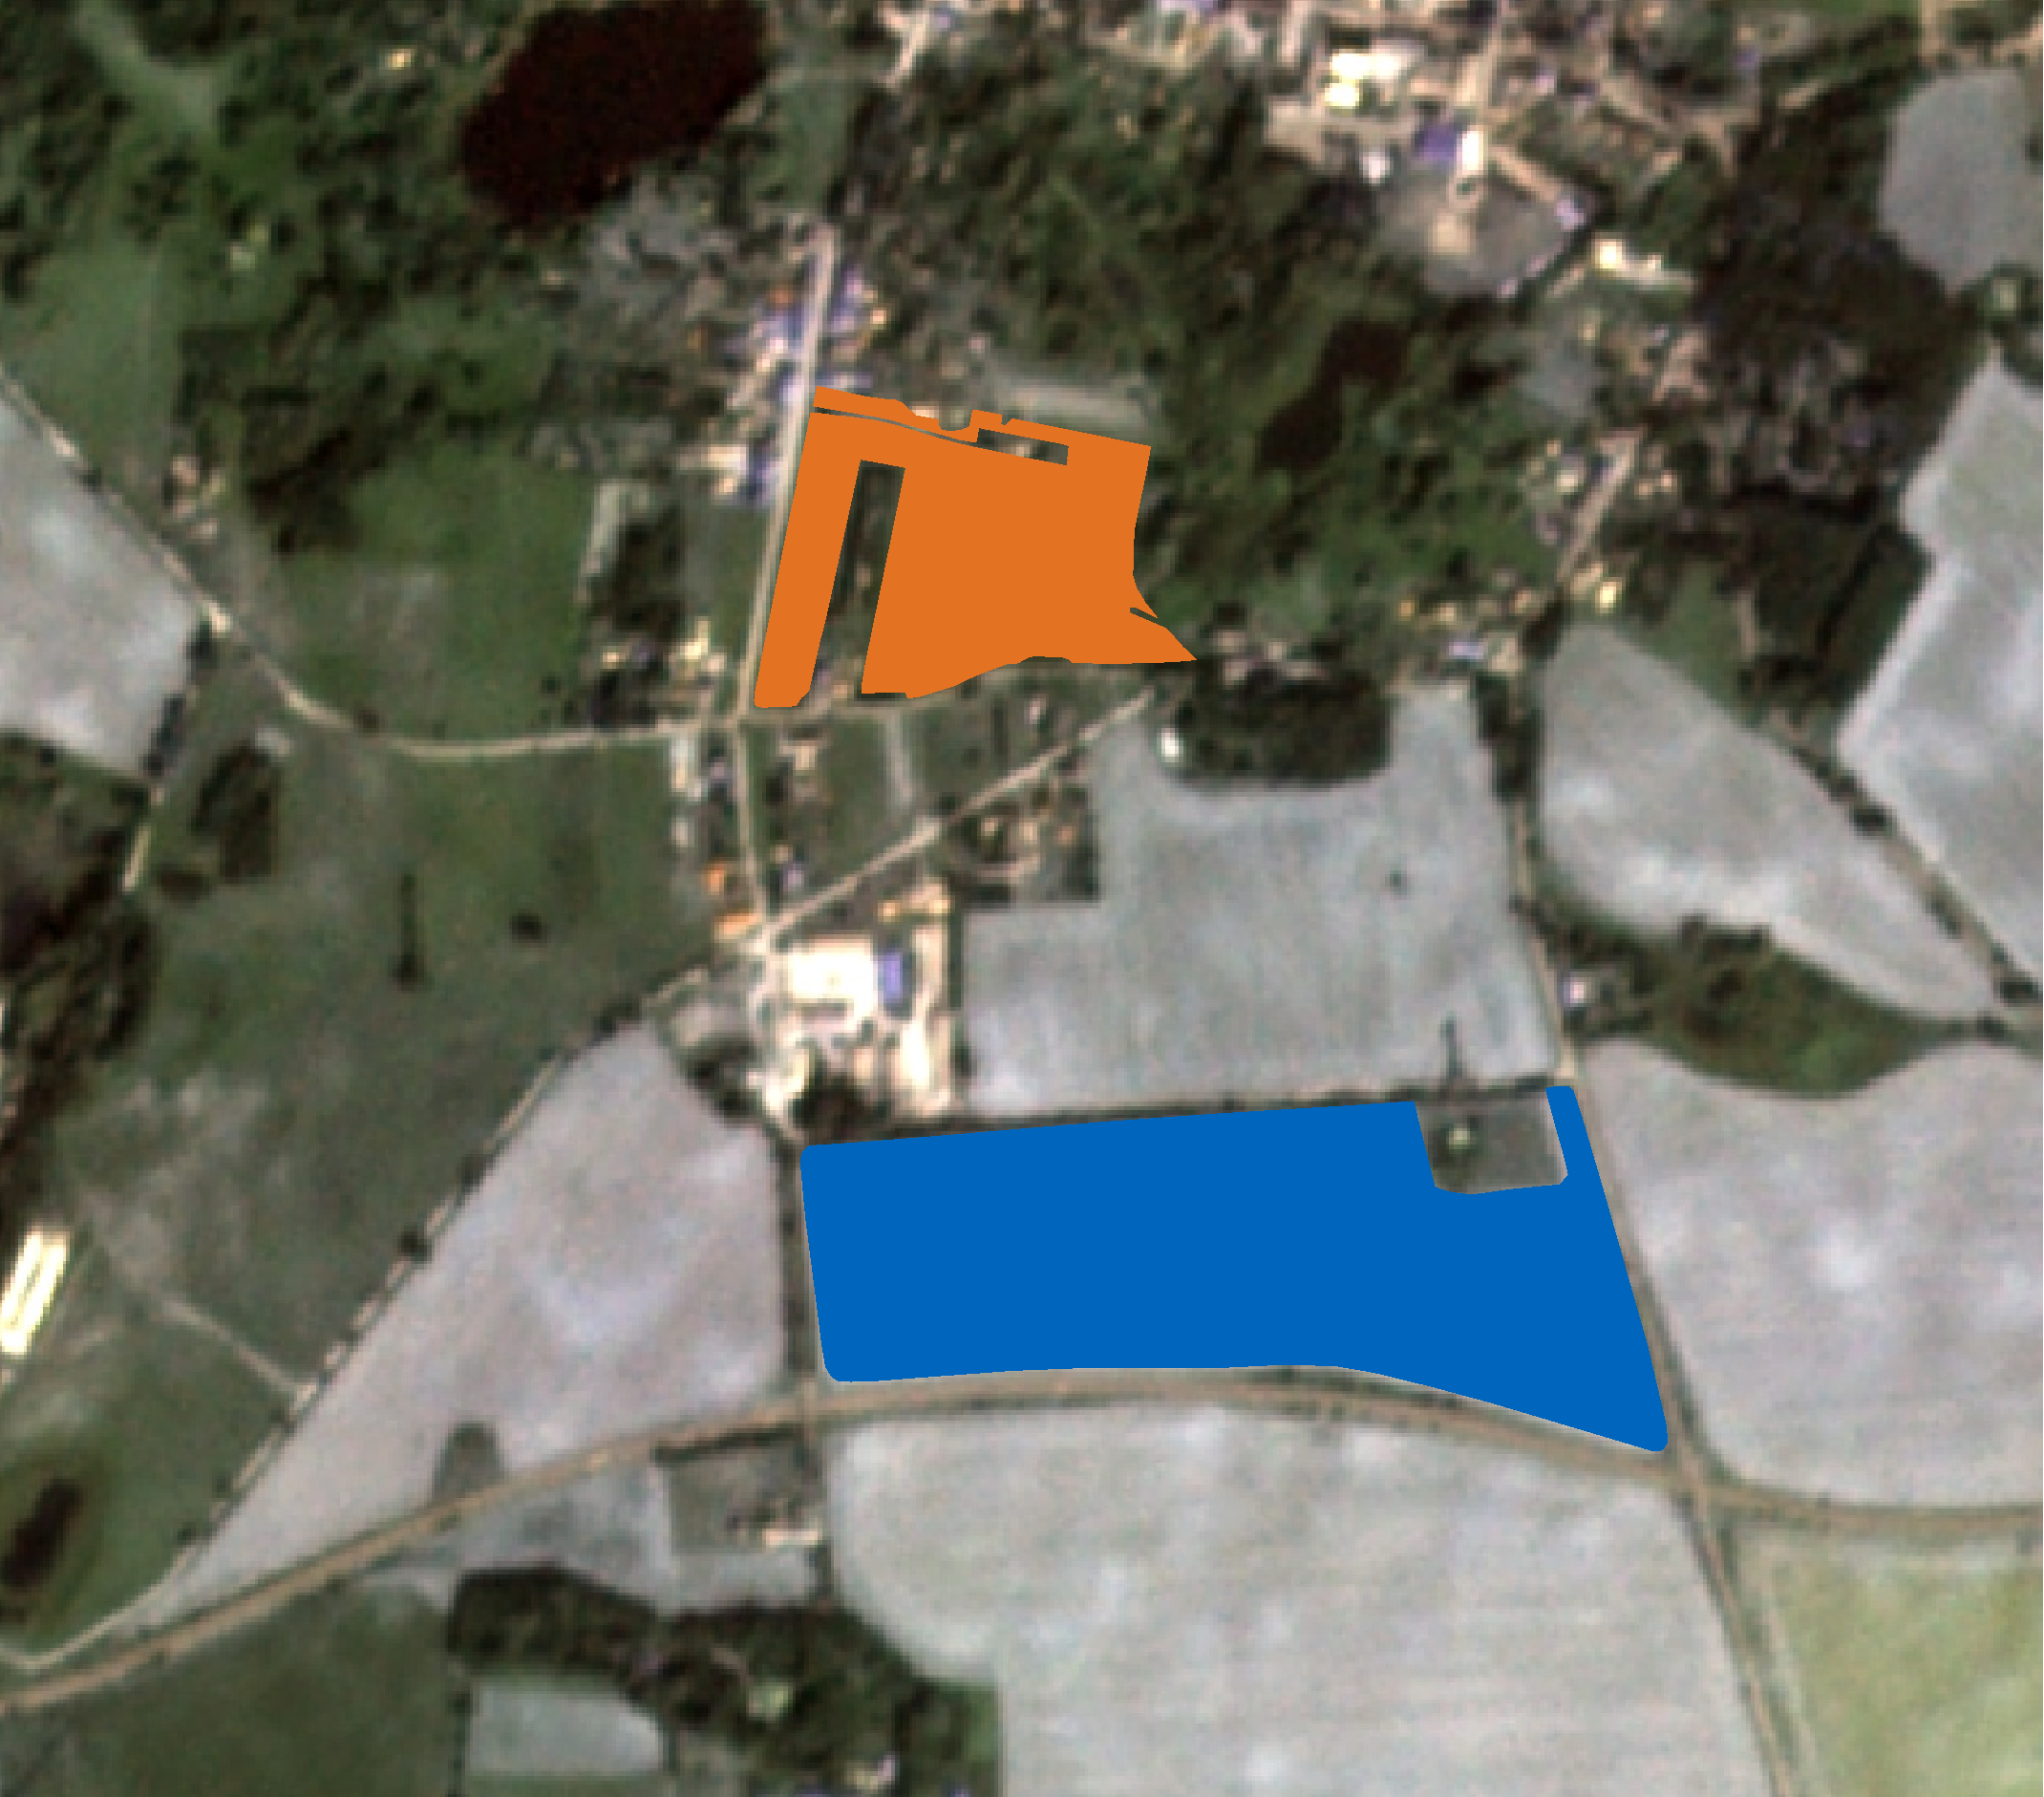
\includegraphics[width=3cm]{images/denethor/map}};
		
		%\node[below=of c]{\includegraphics[width=.9\textwidth]{images/plotss2}};
		
		\definecolor{mpldefaultblue}{HTML}{1f77b4}
		%\coodinate (l1) at ($ (c) + (1,1) $);
%		\draw[Circle - , color=mpldefaultblue] ($ (c) + (-.45,1.6) $) -- ($ (b) + (-3.8,-.8) $); % requires \usetikzlibrary{arrows.meta} and calc
%		\draw[Circle - , color=mpldefaultblue] ($ (c) + (.78,1.6) $) -- ($ (b) + (-1.4,-.8) $);
%		\draw[Circle - , color=mpldefaultblue] ($ (c) + (1.38,1.6) $) -- ($ (b) + (1.6,-.8) $);
%		\draw[Circle - , color=mpldefaultblue] ($ (c) + (2.46,1.6) $) -- ($ (b) + (5,-.8) $);
		
		%\node[circle, draw] at (l1) {+};
		
		\end{tikzpicture}
		
		\citeapa{Kondmann, et al., "DENETHOR: The DynamicEarthNET dataset for Harmonized, inter-Operable, analysis-Ready, daily crop monitoring from space.". NeurIPS Data Track (2021).}
	\end{frame}

	\begin{frame}{Model-Driven Methods}
		\begin{columns}
			\column{.5\textwidth}
				\resizebox{\textwidth}{!}{
					\begin{tikzpicture}
					\node[label={above:\scriptsize growth stages of corn Mimic et al 2020}, inner sep=0](a){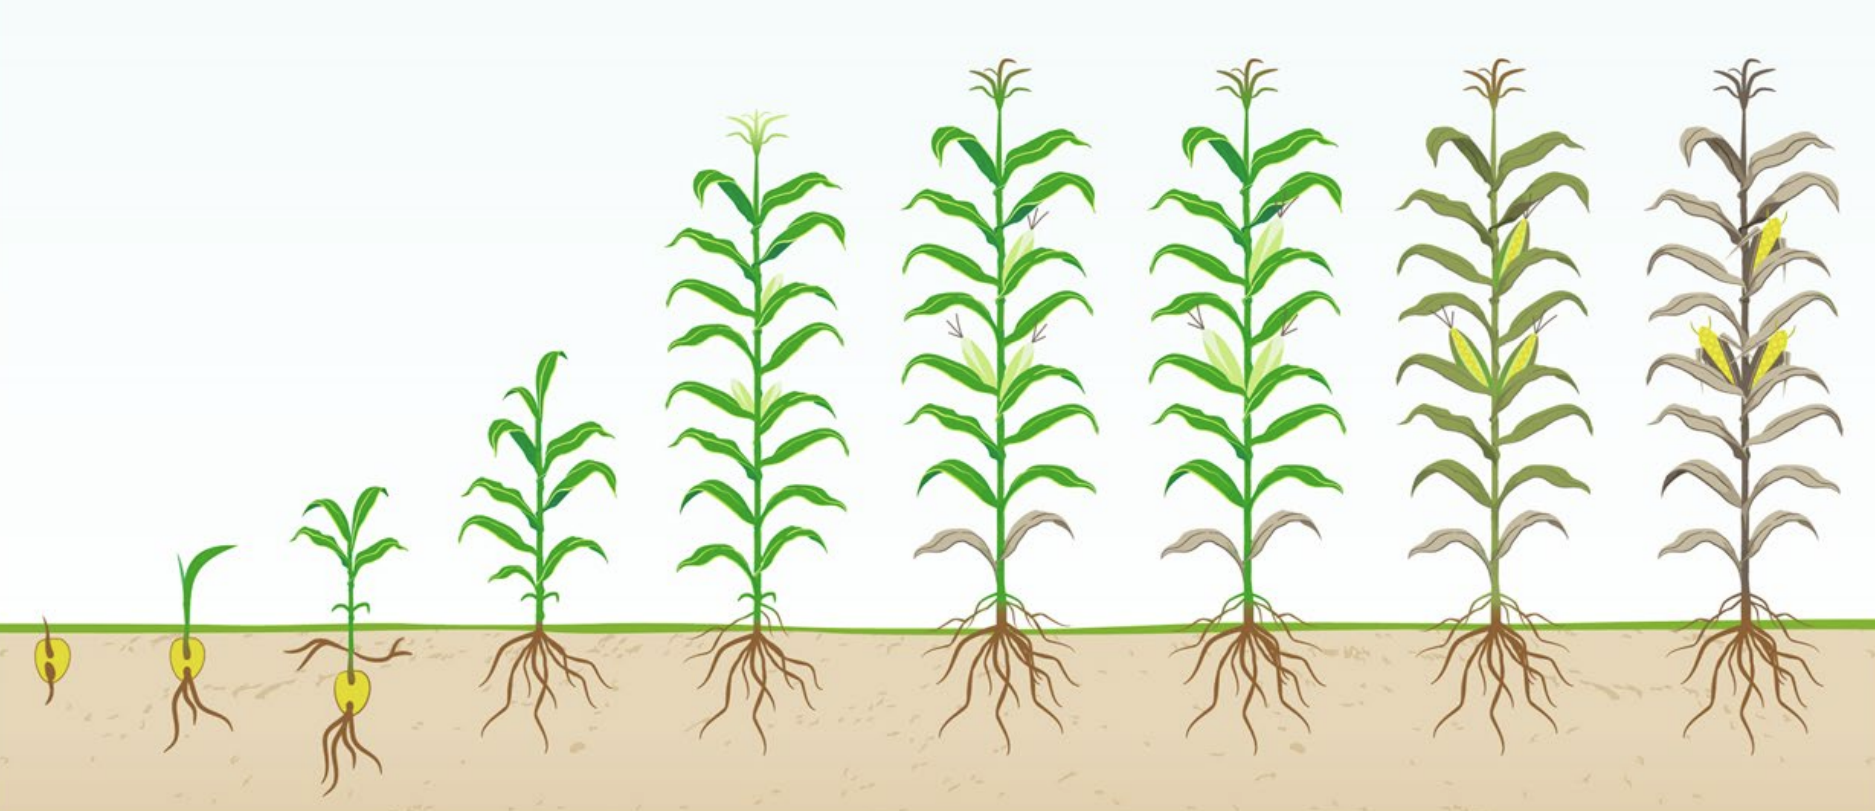
\includegraphics[width=6cm]{images/example/mimicetal2020_phenology_maize_}};
					
					\node[below=1em of a] (b){\includegraphics{images/example/NDVI}};
					
					\coordinate(left)  at ($(a.south west)+(-4.3em,0)$);
					\coordinate(right) at ($(a.south east)+(1.1em,0)$);
					
					\coordinate(veannot) at ($(left)!0.22!(right)$){};
					\coordinate(vtwoannot) at ($(left)!0.275!(right)$){};
					\coordinate(vfiveannot) at ($(left)!0.34!(right)$){};
					\coordinate(vtenannot) at ($(left)!0.42!(right)$){};
					\coordinate(btnnot) at ($(left)!0.5!(right)$){};
					\coordinate(rtwoannot) at ($(left)!0.6!(right)$){};
					\coordinate(rthreeannot) at ($(left)!0.7!(right)$){};
					\coordinate(rfiveannot) at ($(left)!0.8!(right)$){};
					\coordinate(harvestannot) at ($(left)!0.9!(right)$){};
					
					\coordinate(ve) at      ($ (b.center)+(-4em  ,1em) $);
					\coordinate(vtwo) at    ($ (b.center)+(-3em  ,1em) $);
					\coordinate(vfive) at   ($ (b.center)+(-2.5em,3em) $);
					\coordinate(vten) at    ($ (b.center)+(-2em  ,4em) $);
					\coordinate(bt) at      ($ (b.center)+(-1.5em,4.5em) $);
					\coordinate(rtwo) at    ($ (b.center)+(-1em  ,4.5em) $);
					\coordinate(rthree) at  ($ (b.center)+(-0em  ,2em) $);
					\coordinate(rfive) at   ($ (b.center)+(1.5em ,0.5em) $);
					\coordinate(harvest) at ($ (b.center)+(3em   ,0.5em) $);
					
					\draw[Circle-,tumorange](veannot)      -- (ve);
					\draw[Circle-,tumorange](vtwoannot)    -- (vtwo);
					\draw[Circle-,tumorange](vfiveannot)   -- (vfive);
					\draw[Circle-,tumorange](vtenannot)    -- (vten);
					\draw[Circle-,tumorange](btnnot)       -- (bt);
					\draw[Circle-,tumorange](rtwoannot)    -- (rtwo);
					\draw[Circle-,tumorange](rthreeannot)  -- (rthree);
					\draw[Circle-,tumorange](rfiveannot)   -- (rfive);
					\draw[Circle-,tumorange](harvestannot) -- (harvest);
					\end{tikzpicture}
				}
			\column{.5\textwidth}
				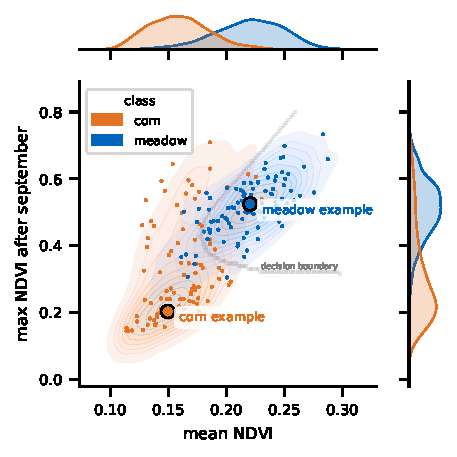
\includegraphics[width=\textwidth]{images/example/jointplot}
			
		\end{columns}
	
		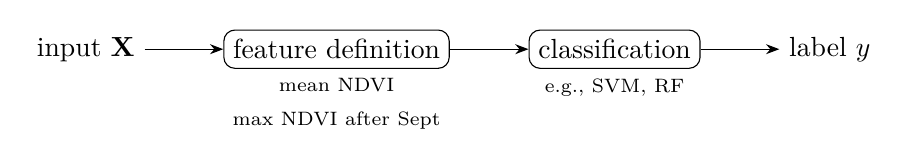
\begin{tikzpicture}
			\tikzstyle{process} = [draw, rounded corners]
			\node(x){input $\mathbf{X}$};
			\node[process, right=of x](f){feature definition};
			\node[process, right=of f](c){classification};
			\node[right=of c](y){label $y$};
			\draw[-Stealth](x) -- (f);
			\draw[-Stealth](f) -- (c);
			\draw[-Stealth](c) -- (y);
			\node[below=0cm of f, font=\scriptsize](a){mean NDVI};
			\node[below=0cm of a, font=\scriptsize](b){max NDVI after Sept};
			
			\node[below=0cm of c, font=\scriptsize](a){e.g., SVM, RF};
		\end{tikzpicture}
		
	\end{frame}

	
	\newcommand{\nn}{
		\tikzstyle{proba} = [circle, draw=white, inner sep=2.5pt, fill=rouge]
		\begin{tikzpicture}[scale=0.5, rotate=0, baseline=-.25em, minimum width=0cm, minimum height=0cm]
		\node[proba](a0) at (0,-1){};
		\node[proba](a1) at (0,0){};
		\node[proba](a2) at (0,1){};
		
		\node[proba](b0) at (1,-0.5){};
		\node[proba](b1) at (1,0.5){};
		
		\draw[-] (a0) -- (b0);
		\draw[-] (a1) -- (b0);
		\draw[-] (a2) -- (b0);
		
		\draw[-] (a0) -- (b1);
		\draw[-] (a1) -- (b1);
		\draw[-] (a2) -- (b1);
		
		%	\node[fit=(a0)(a2)(b1)](node name){};
		
		\end{tikzpicture}
	}

	\newcommand{\featurelearningtikz}{
		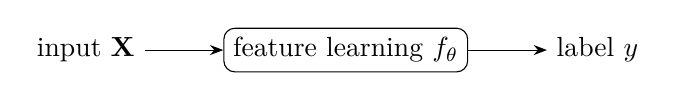
\begin{tikzpicture}
			\tikzstyle{process} = [draw, rounded corners]
			\node(x){input $\mathbf{X}$};
			\node[process, right=of x](f){feature learning $f_\mathbf{\theta}$ \nn};
			\node[right=of f](y){label $y$};
			\draw[-Stealth](x) -- (f);
			\draw[-Stealth](f) -- (y);
		\end{tikzpicture}
	}

	\begin{frame}[t]{Data-Driven Methods}
		
		
		\centering
		\featurelearningtikz
		
		\vspace{1em}
		
		\raggedright
		
		\resizebox{\textwidth}{!}{
			\colorlet{tumgray}{gray}
\tikzstyle{annotation} = [font=\small, text width=3.5cm]
\tikzstyle{node} = [circle, draw, font=\small]
\tikzstyle{edge} = [-stealth, tumgray]
\tikzstyle{operation} = [font=\scriptsize, fill=white, text=black]
\tikzstyle{normal} = [font=\scriptsize, text=tumblue]
\begin{tikzpicture}[node distance=0]



\node(a){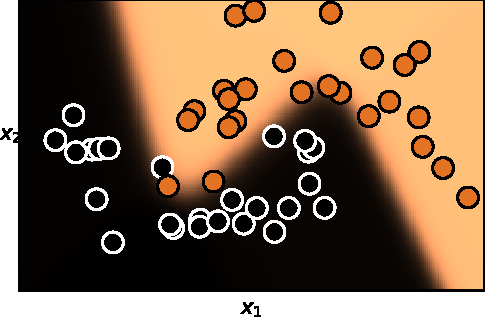
\includegraphics[width=3cm]{nn/x.pdf}};
\node[right=of a](b){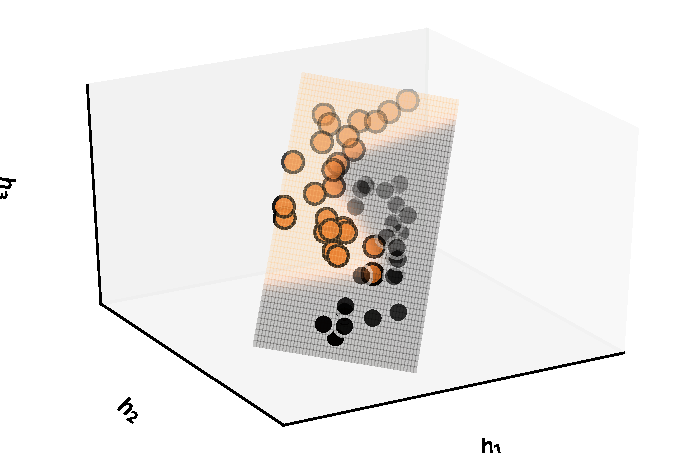
\includegraphics[width=4.5cm]{nn/h.pdf}};
\node[right=of b](c){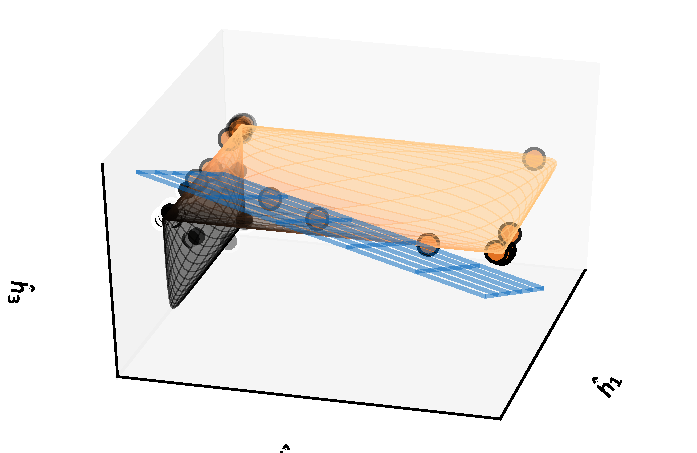
\includegraphics[width=4.5cm]{nn/h2.pdf}};
\node[right=1em of c](d){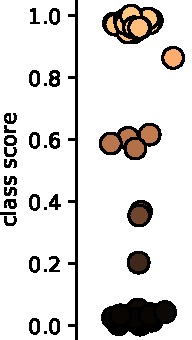
\includegraphics[width=1.2cm]{nn/y.pdf}};

\coordinate(annotations) at (0,-3);
\node[annotation] at (a |- annotations){(a) Input space \\ $\mathbf{x} = (x_1, x_2)$};
\node[annotation] at (b |- annotations){(b) linear projection $\mathbf{w}_1^T\mathbf{x}$ into $\mathbb{R}^3$};
\node[annotation, xshift=-2em] at (c |- annotations){(c) non-linear distortion with $\tanh(\mathbf{w}_1^T\mathbf{x})$};
\node[annotation] at (d |- annotations){(d) Output class probabilities $y \in [0,1]$};

\coordinate(network) at (0,3);
\coordinate(networklone) at (a |- network);
\coordinate(networkltwo) at (b |- network);
\coordinate(networklthree) at (c |- network);
\coordinate(networklast) at (d |- network);

\node[node, above=of networklone](xone){$x_1$};
\node[node, below=of networklone](xtwo){$x_2$};
\begin{scope}[node distance=1.3em]
\node[node, above=of networkltwo](hone){$h_1$};
\node[node] at (networkltwo)(htwo){$h_2$};
\node[node, below=of networkltwo](hthree){$h_3$};
\end{scope}

\begin{scope}[node distance=1.3em]
\node[node, above=of networklthree](hhone){$\hat{h}_1$};
\node[node] at (networklthree)(hhtwo){$\hat{h}_2$};
\node[node, below=of networklthree](hhthree){$\hat{h}_3$};
\end{scope}

%			\node[node] at (networklthree){a};
\node[node](y) at (networklast){$y$};

\draw[edge] (xone) -- (hone);
\draw[edge] (xone) -- (htwo);
\draw[edge] (xone) -- (hthree);
\node[operation] at ($(networklone)!0.5!(networkltwo)$) {$\mathbf{W}_1$};

\draw[edge] (xtwo) -- (hone);
\draw[edge] (xtwo) -- (htwo);
\draw[edge] (xtwo) -- (hthree);

\draw[edge] (hone) -- node[midway]{} (hhone);
\draw[edge] (htwo) -- node[midway, operation]{$\tanh$} (hhtwo);
\draw[edge] (hthree) -- node[midway]{} (hhthree);

\draw[edge] (hhthree) -- node[near start, below, normal, name=lastweight]{$w_{2,3}$} (y);
\draw[edge] (hhone) -- node[near start, below, normal]{$w_{2,1}$} (y);
\draw[edge] (hhtwo) -- node[near start, below, normal]{$w_{2,2}$} node[near end, operation]{$\Sigma \circ \sigma$} (y);

\draw[-stealth, tumblue] (lastweight) to[bend left] node[near start, yshift=1em, right, font=\tiny, text width=3.5cm]{$\mathbf{w}_2 = (w_{2,1},w_{2,2},w_{2,3})$ defines the normal of the decision plane} ++(-1,-2);

%\draw[decorate, decoration = {brace}] ($(networklone)+(0,4em)$) -- node[midway, above, font=\small]{feature extraction} ($(networklthree)+(0,4em)$);
%\draw[decorate, decoration = {brace}] ($(networklthree)+(0,4em)$) -- node[midway, above, font=\small]{classification} ($(networklast)+(0,4em)$);

\end{tikzpicture}
		}
	\end{frame}

	\begin{frame}[t]{Data-Driven Methods}
		\centering
		\featurelearningtikz
		
		\hspace{-1em} Search for suitable data-specific architecture
			
			\begin{columns}[t]
				
				\column{.5\textwidth}
				
				In general
					\begin{itemize}
						\item CNNs for images (e.g. ResNet50)
						\item Transformers/RNNs for language (e.g. Bert)
					\end{itemize}
				\column{.5\textwidth}
				
				For crop type mapping
				\begin{itemize}
					\item CNNs 
					\item RNNs 
					\item Transformers
				\end{itemize}
			\end{columns}
		
		\vspace{2em}
			\centering
			{Data-driven deep learning models are very plastic and (blindly) learn to approximate target data.}\\
			
			\vspace{1em}
			We need to think carefully how we sample and select data. 
			
	\end{frame}

	\newcommand{\iidsim}{\mathrel{\overset{\makebox[0pt]{\mbox{\normalfont\tiny\sffamily i.i.d}}}{\sim}}}
	\begin{frame}[t]{Data Generation Model}
		\centering
%		
%		\featurelearningtikz
%		
%		\vspace{1em}
		
		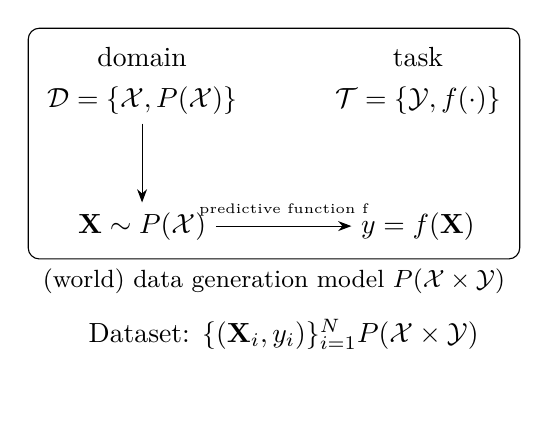
\begin{tikzpicture}
			\node[label={[name=domainlabel]domain}](domain){$\mathcal{D} = \{\mathcal{X}, P(\mathcal{X})\}$};
			\node[label={[name=tasklabel]task}, right=of domain](task){$\mathcal{T} = \{\mathcal{Y}, f(\cdot)\}$};
			
			\node[below=of domain](xsample){$\mathbf{X} \sim P(\mathcal{X})$};
			
			\node[below=of task](ysample){$y = f(\mathbf{X})$};
			
			\draw[-Stealth] (domain) -- (xsample);
			\draw[-Stealth] (xsample) -- node[midway, above, font=\tiny, name=label]{predictive function f} (ysample);
			
			\node[fit=(domain)(xsample)(task)(ysample)(domainlabel)(tasklabel), draw, rounded corners, label={[name=dgm, font=\small]below:(world) data generation model $P(\mathcal{X} \times \mathcal{Y})$}](box) {};
%			\node[right=of box, font]{Data Generation Model};

			
			\node[below=3em of label](datasampling){Dataset: $\{(\mathbf{X}_i,y_i)\}_{i=1}^N \iidsim P(\mathcal{X} \times \mathcal{Y})$};
			
			\node[below=1em of datasampling](model){\featurelearningtikz};
			
		\end{tikzpicture}
		\vfill\tiny
		\citeapa{Pan, S. J., \& Yang, Q. (2009). A survey on transfer learning. IEEE Transactions on knowledge and data engineering, 22(10), 1345-1359.}
		\citeapa{Qiang Yang; Yu Zhang, Wenyuan Dai; Sinno Jialin Pan (Editors) (2020). Transfer learning. Cambridge University Press. DOI 9781139061773}
		\citeapa{Shai Ben-David and Shai Shalev-Shwartz (2014). Understanding Machine Learning: From Theory to Algorithms}
	\end{frame}

	
	\begin{frame}
		\frametitle{I.I.D assumption}
		
		we use a dataset $\{(\mathbf{X}_i,y_i)\}_{i=1}^N \iidsim P(\mathcal{X} \times \mathcal{Y})$ of \textbf{independently} and and \textbf{identically} distributed (i.i.d) samples.
		\vspace{1em}
		
		\pause
		we need \textbf{independence} for the factorization in max likelihood.
		\begin{align*}
		\theta^\ast &= \arg\max_\theta \prod_{i} p(y_i \vert \mathbf{X}_i)  \\
		&= \arg\min_\theta \sum_{i} -y_i \log f_\theta(\mathbf{X}_i)
		\end{align*}
		
		\pause
		we assume an \textbf{identical distribution} $P(\mathcal{X} \times \mathcal{Y})$ throughout the entire data generation { \scriptsize (and particularly between training and test time) }
		\begin{align}
		X_i,y_i \iidsim P(\mathcal{X} \times \mathcal{Y})
		\end{align}
		which implies identical domains $\mathcal{D} = \{\mathcal{X}, P(\mathcal{X})\}$ and tasks $\mathcal{T} = \{\mathcal{Y}, f(\cdot)\}$ during training and test time.
		
	\end{frame}

	\begin{frame}{In- and Out-of-Dist. Generalization}
		
		The I.I.D assumption is usually enforced via random splitting a single dataset $D$ into training and testing partitions
		
		\vspace{2em}
		
		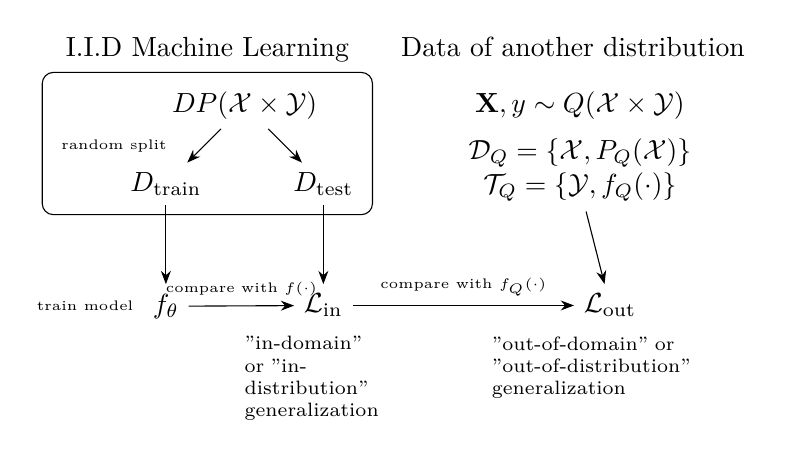
\begin{tikzpicture}
			\node(ds) at (0,0){$D \iidsim P(\mathcal{X} \times \mathcal{Y})$};
			\node at (-1,-1)(dstrain){$D_\text{train}$};
			\node at (1,-1)(dstest){$D_\text{test}$};
			
			\draw[-Stealth](ds) --node[midway, left=1em, font=\tiny, name=labelsplit]{random split} (dstrain);
			\draw[-Stealth](ds) -- (dstest);
			
			\node[draw, rounded corners, fit=(ds)(dstrain)(dstest)(labelsplit), label={above: I.I.D Machine Learning}]{};
			
			\node[below=of dstrain, label={[font=\tiny]left:train model}] (weights) {$f_\theta$};
			\draw[-Stealth] (dstrain) -- (weights);
			
			\node[below=of dstest] (testloss) {$\mathcal{L}_\text{in}$};
			\draw[-Stealth] (dstest) -- (testloss);
			\draw[-Stealth] (weights) -- node[midway,above,font=\tiny]{compare with $f(\cdot)$} (testloss);
			
			\node[below=0em of testloss, text width=2cm, font=\scriptsize](tllabel){"in-domain" or "in-distribution" generalization};
			
			\visible<2->{
				\node[right=5em of ds](Q){$\mathbf{X},y \sim Q(\mathcal{X} \times \mathcal{Y})$};
				
				\node[below=0em of Q](domain){$\mathcal{D}_Q = \{\mathcal{X}, P_Q(\mathcal{X})\}$};
				\node[below=-.5em of domain](task){$\mathcal{T}_Q = \{\mathcal{Y}, f_Q(\cdot)\}$};
				
				\node[rounded corners, fit=(Q)(domain)(task), label={above: Data of another distribution\phantom{g}}]{};
				
				\node[right=8em of testloss] (oodloss) {$\mathcal{L}_\text{out}$};
				\node[below=0em of oodloss, text width=3cm, font=\scriptsize](oodlabel){"out-of-domain" or \\ "out-of-distribution" \\ generalization};
				
				\draw[-Stealth] (testloss) -- node[midway,above,font=\tiny]{compare with $f_Q(\cdot)$} (oodloss);
				\draw[-Stealth] (task) -- (oodloss);
			}
		\end{tikzpicture}
	\end{frame}

	\begin{frame}{Measuring OOD Generalization}
		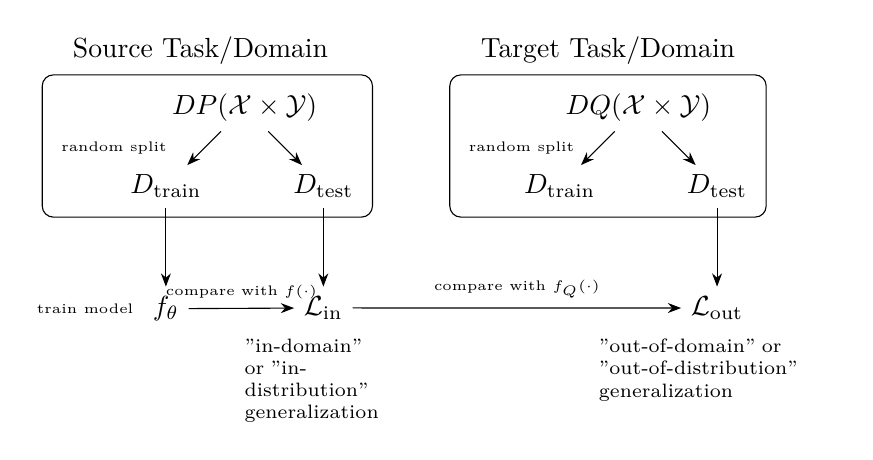
\begin{tikzpicture}
		\node(ds) at (0,0){$D \iidsim P(\mathcal{X} \times \mathcal{Y})$};
		\node at (-1,-1)(dstrain){$D_\text{train}$};
		\node at (1,-1)(dstest){$D_\text{test}$};
		
		\draw[-Stealth](ds) --node[midway, left=1em, font=\tiny, name=labelsplit]{random split} (dstrain);
		\draw[-Stealth](ds) -- (dstest);
		
		\node[draw, rounded corners, fit=(ds)(dstrain)(dstest)(labelsplit), label={above: Source Task/Domain\phantom{g}}]{};
		
		\node[below=of dstrain, label={[font=\tiny]left:train model}] (weights) {$f_\theta$};
		\draw[-Stealth] (dstrain) -- (weights);
		
		\node[below=of dstest] (testloss) {$\mathcal{L}_\text{in}$};
		\draw[-Stealth] (dstest) -- (testloss);
		\draw[-Stealth] (weights) -- node[midway,above,font=\tiny]{compare with $f(\cdot)$} (testloss);
		
		\node[below=0em of testloss, text width=2cm, font=\scriptsize](tllabel){"in-domain" or "in-distribution" generalization};
		
		\begin{scope}[xshift=5cm]
			\node(Q) at (0,0){$D \iidsim Q(\mathcal{X} \times \mathcal{Y})$};
			\node at (-1,-1)(dsqtrain){$D_\text{train}$};
			\node at (1,-1)(dsqtest){$D_\text{test}$};
		\end{scope}
		
		\draw[-Stealth](Q) --node[midway, left=0.5em, font=\tiny, name=labelqsplit]{random split} (dsqtrain);
		\draw[-Stealth](Q) -- (dsqtest);
		
		\node[draw, rounded corners, fit=(Q)(dsqtrain)(dsqtest)(labelqsplit), label={above: Target Task/Domain}]{};
		
		\node[below=of dsqtest] (oodloss) {$\mathcal{L}_\text{out}$};
		\node[below=0em of oodloss, text width=3cm, font=\scriptsize](oodlabel){"out-of-domain" or \\ "out-of-distribution" \\ generalization};
		
		\draw[-Stealth] (testloss) -- node[midway,above,font=\tiny]{compare with $f_Q(\cdot)$} (oodloss);
		\draw[-Stealth] (dsqtest) -- (oodloss);
		
		\end{tikzpicture}
	\end{frame}

	\begin{frame}{Train/Test Dists are usually not identical}
		
		Examples
		\begin{columns}[t]
			\column{.5\textwidth}
				
				gender classification \\
				{\scriptsize (Buolamwini \& Gebru, 2016)}
				
				\vspace{1em}
				
				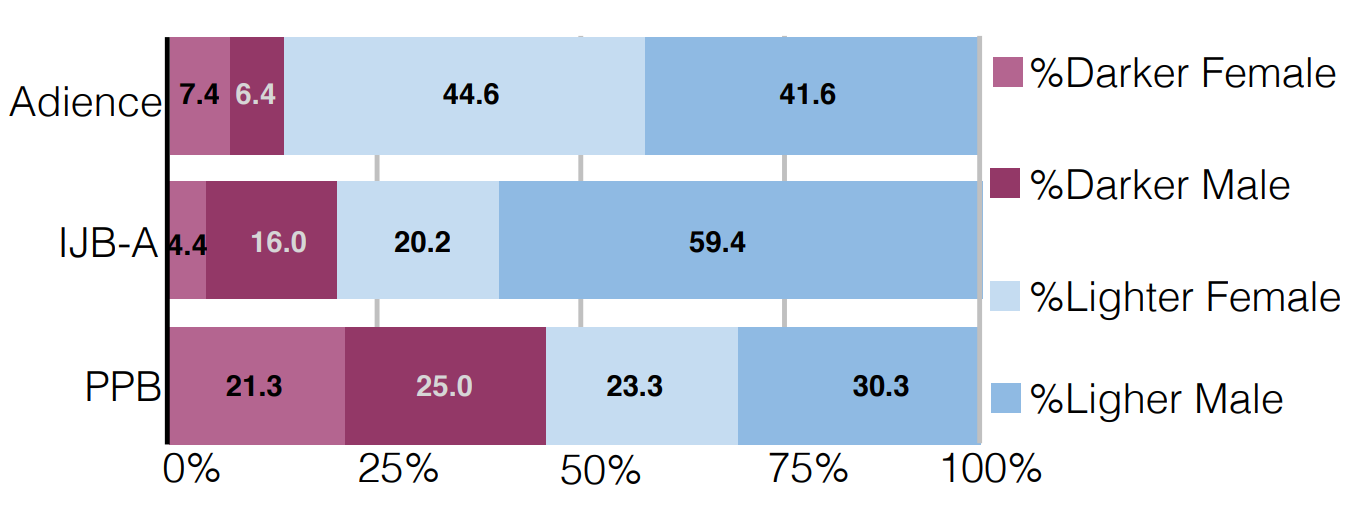
\includegraphics[width=\textwidth]{images/BoulamwiniGebru2016}
				
				\vspace{1em}
				
				CV classifiers performed
				\begin{itemize}
					\item worst for darker females
					\item best for lighter males
				\end{itemize}
			
			\column{.5\textwidth}
			
				large language models
				
				\begin{itemize}
					\item Trained on massive text datasets on the internet (e.g. Reddit).
					\item deployed in everyday situations (e.g. drafting sport aricles/blog posts).
				\end{itemize}
			
				Strereotyp-bias is encoded via the training dataset and can be quantified {\scriptsize (Nadeem et al., 2020)}
			
		\end{columns}
		
		\vfill
	
		\citeapa{Buolamwini, J., \& Gebru, T. (2018, January). Gender shades: Intersectional accuracy disparities in commercial gender classification. In Conference on fairness, accountability and transparency (pp. 77-91). PMLR.}
		
		\citeapa{Nadeem, M., Bethke, A., \& Reddy, S. (2020). Stereoset: Measuring stereotypical bias in pretrained language models. arXiv preprint arXiv:2004.09456.}
	\end{frame}

	\begin{frame}{Distributions shift with location and time}
		\begin{columns}[t]
			\column{.5\textwidth}
			Dominant crop type (by color)
			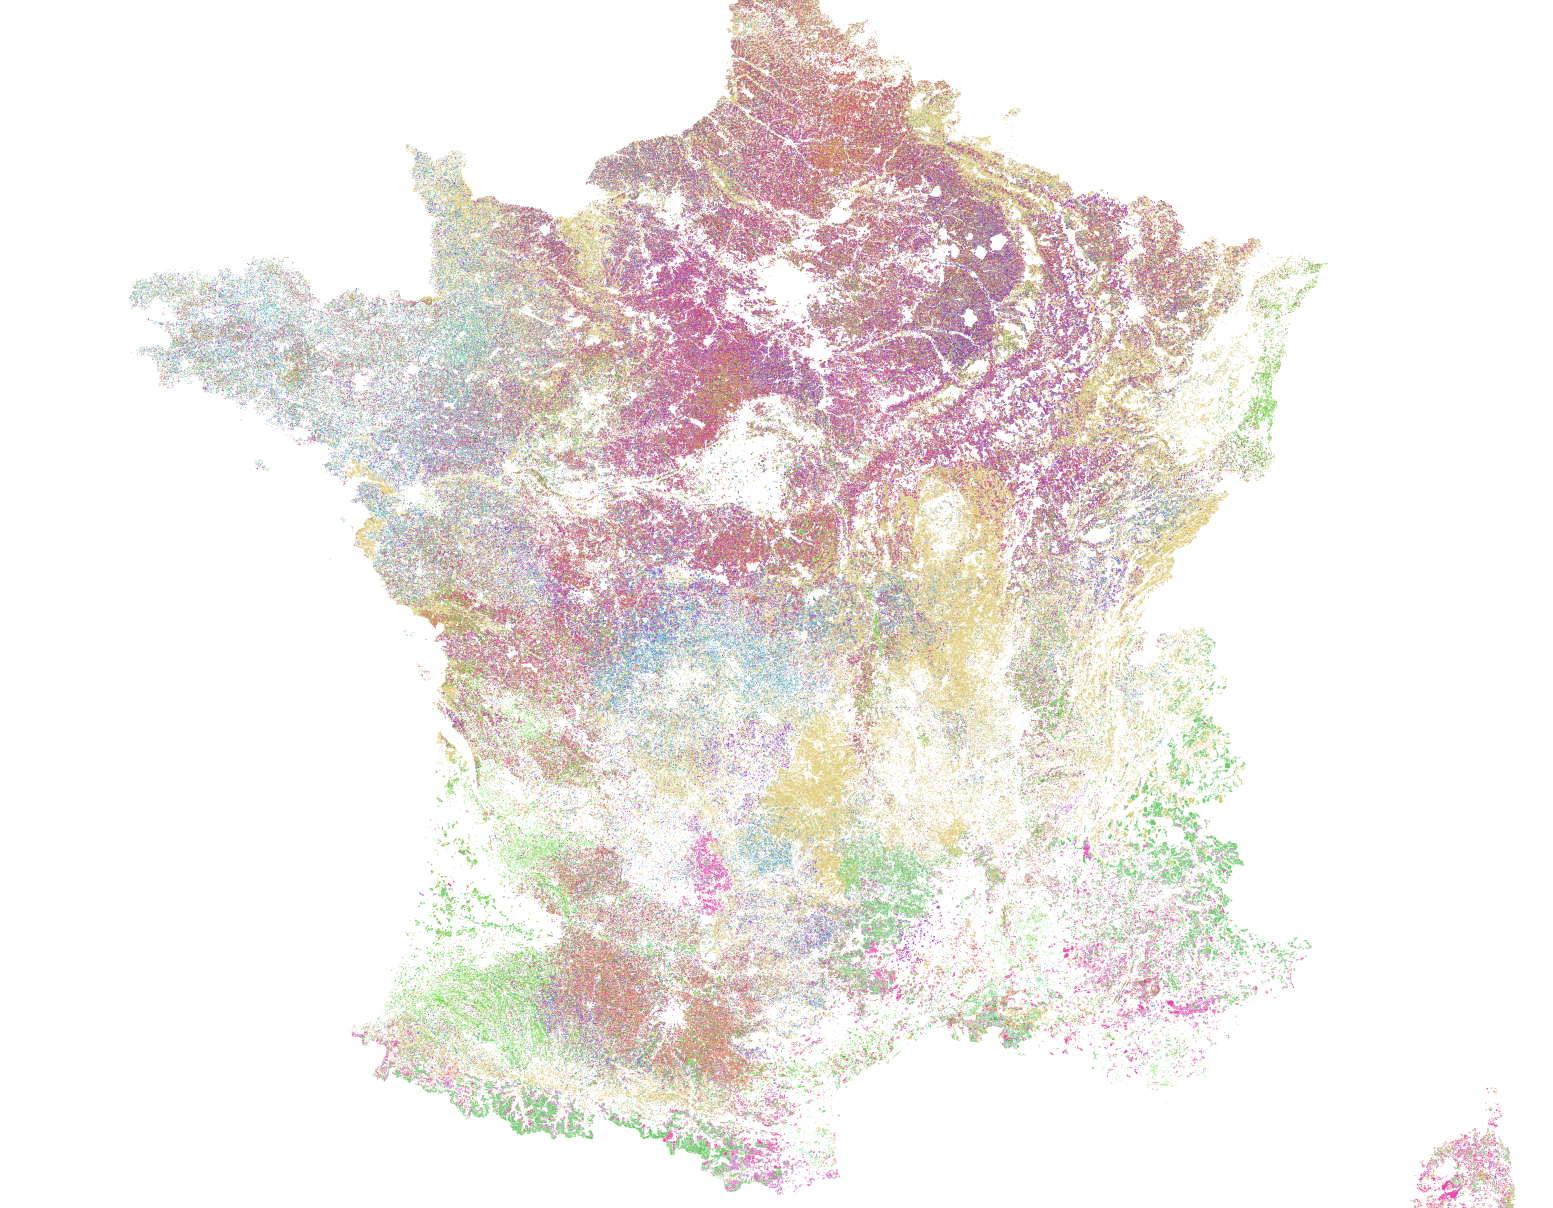
\includegraphics[width=\textwidth]{images/france_crop_distribution}
			
			\column{.5\textwidth}
			\only<2>{
			Max temp (23-30°C) 2018-08
			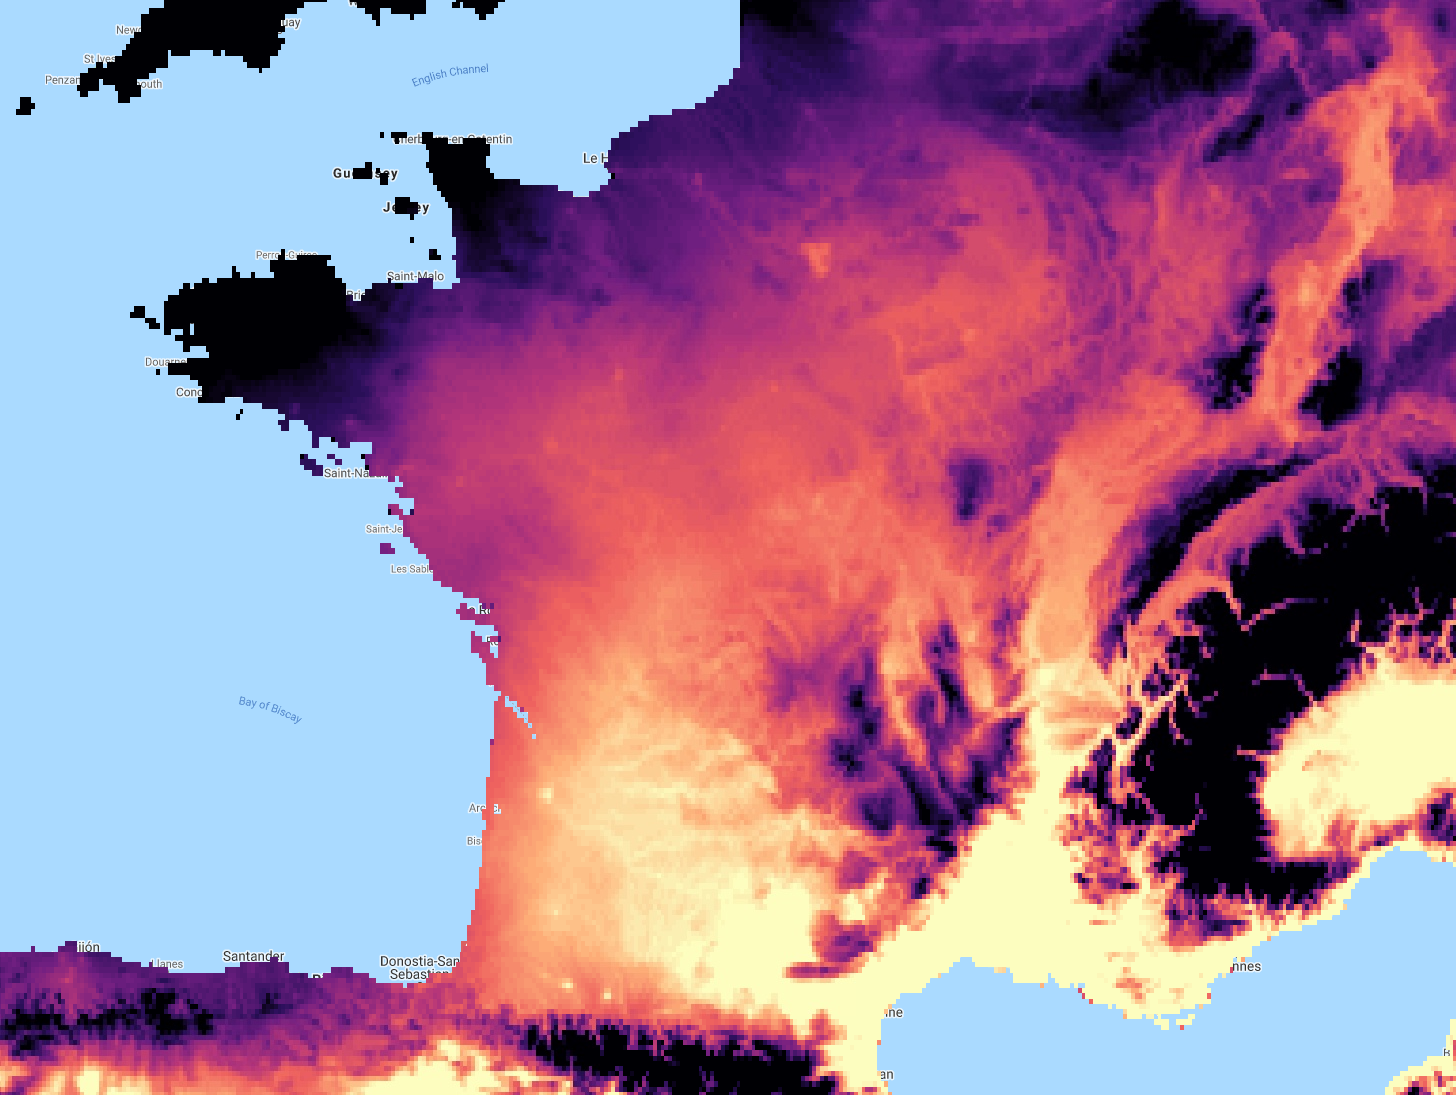
\includegraphics[width=\textwidth]{images/france_tmmx_201808}
			}
			\only<3>{
				Precipitation 2018-08
				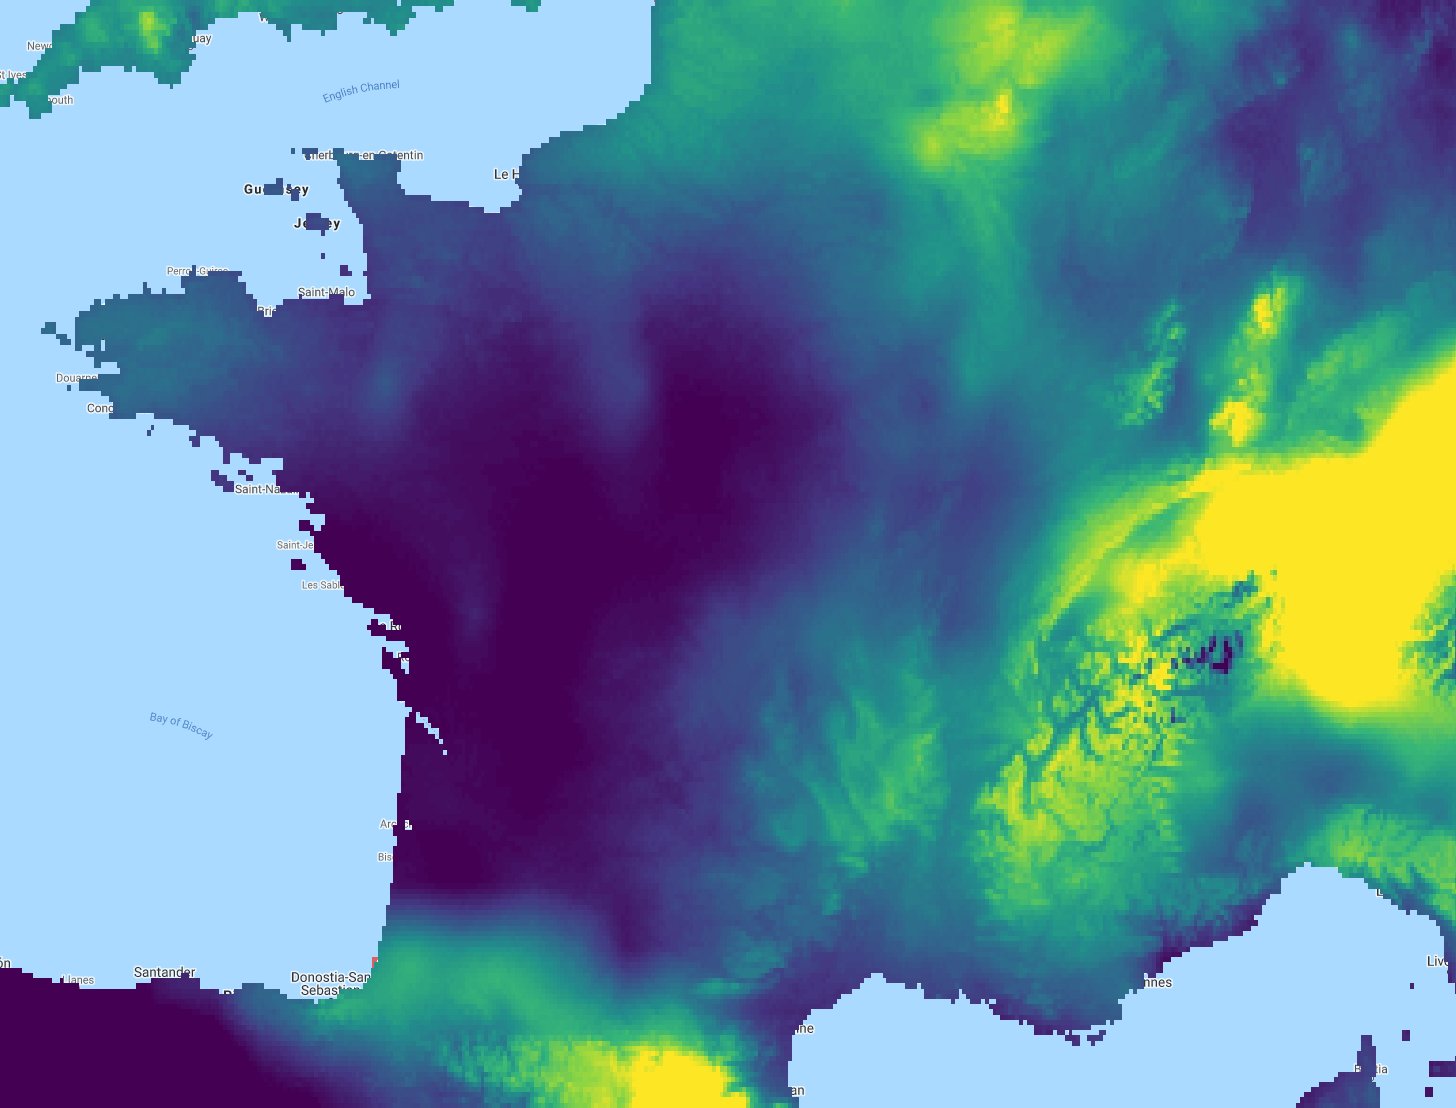
\includegraphics[width=\textwidth]{images/france_pr_201808}
			}
		\end{columns}
	\end{frame}


	\begin{frame}{Toy Example: "wheat" vs "other cereals"}
		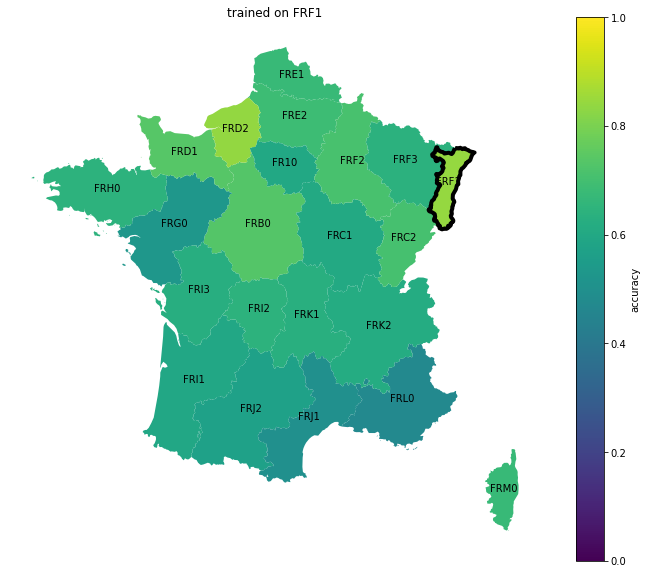
\includegraphics[width=.49\textwidth]{images/francecrops/frf1.png}
		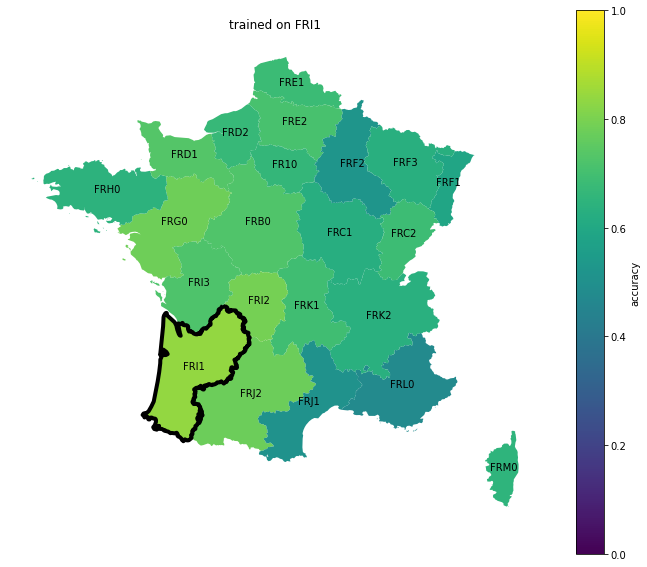
\includegraphics[width=.49\textwidth]{images/francecrops/fri1.png}
		
		\vspace{1em}
		binary "wheat" vs "other cereals" classification
		
		\vspace{1em}
		{\small 
			crop type time series classification with a simple 1D-CNN and 200 samples per class	in each NUTS-2 region
		}
	\end{frame}



	\begin{frame}{Global Distribution Shift}
		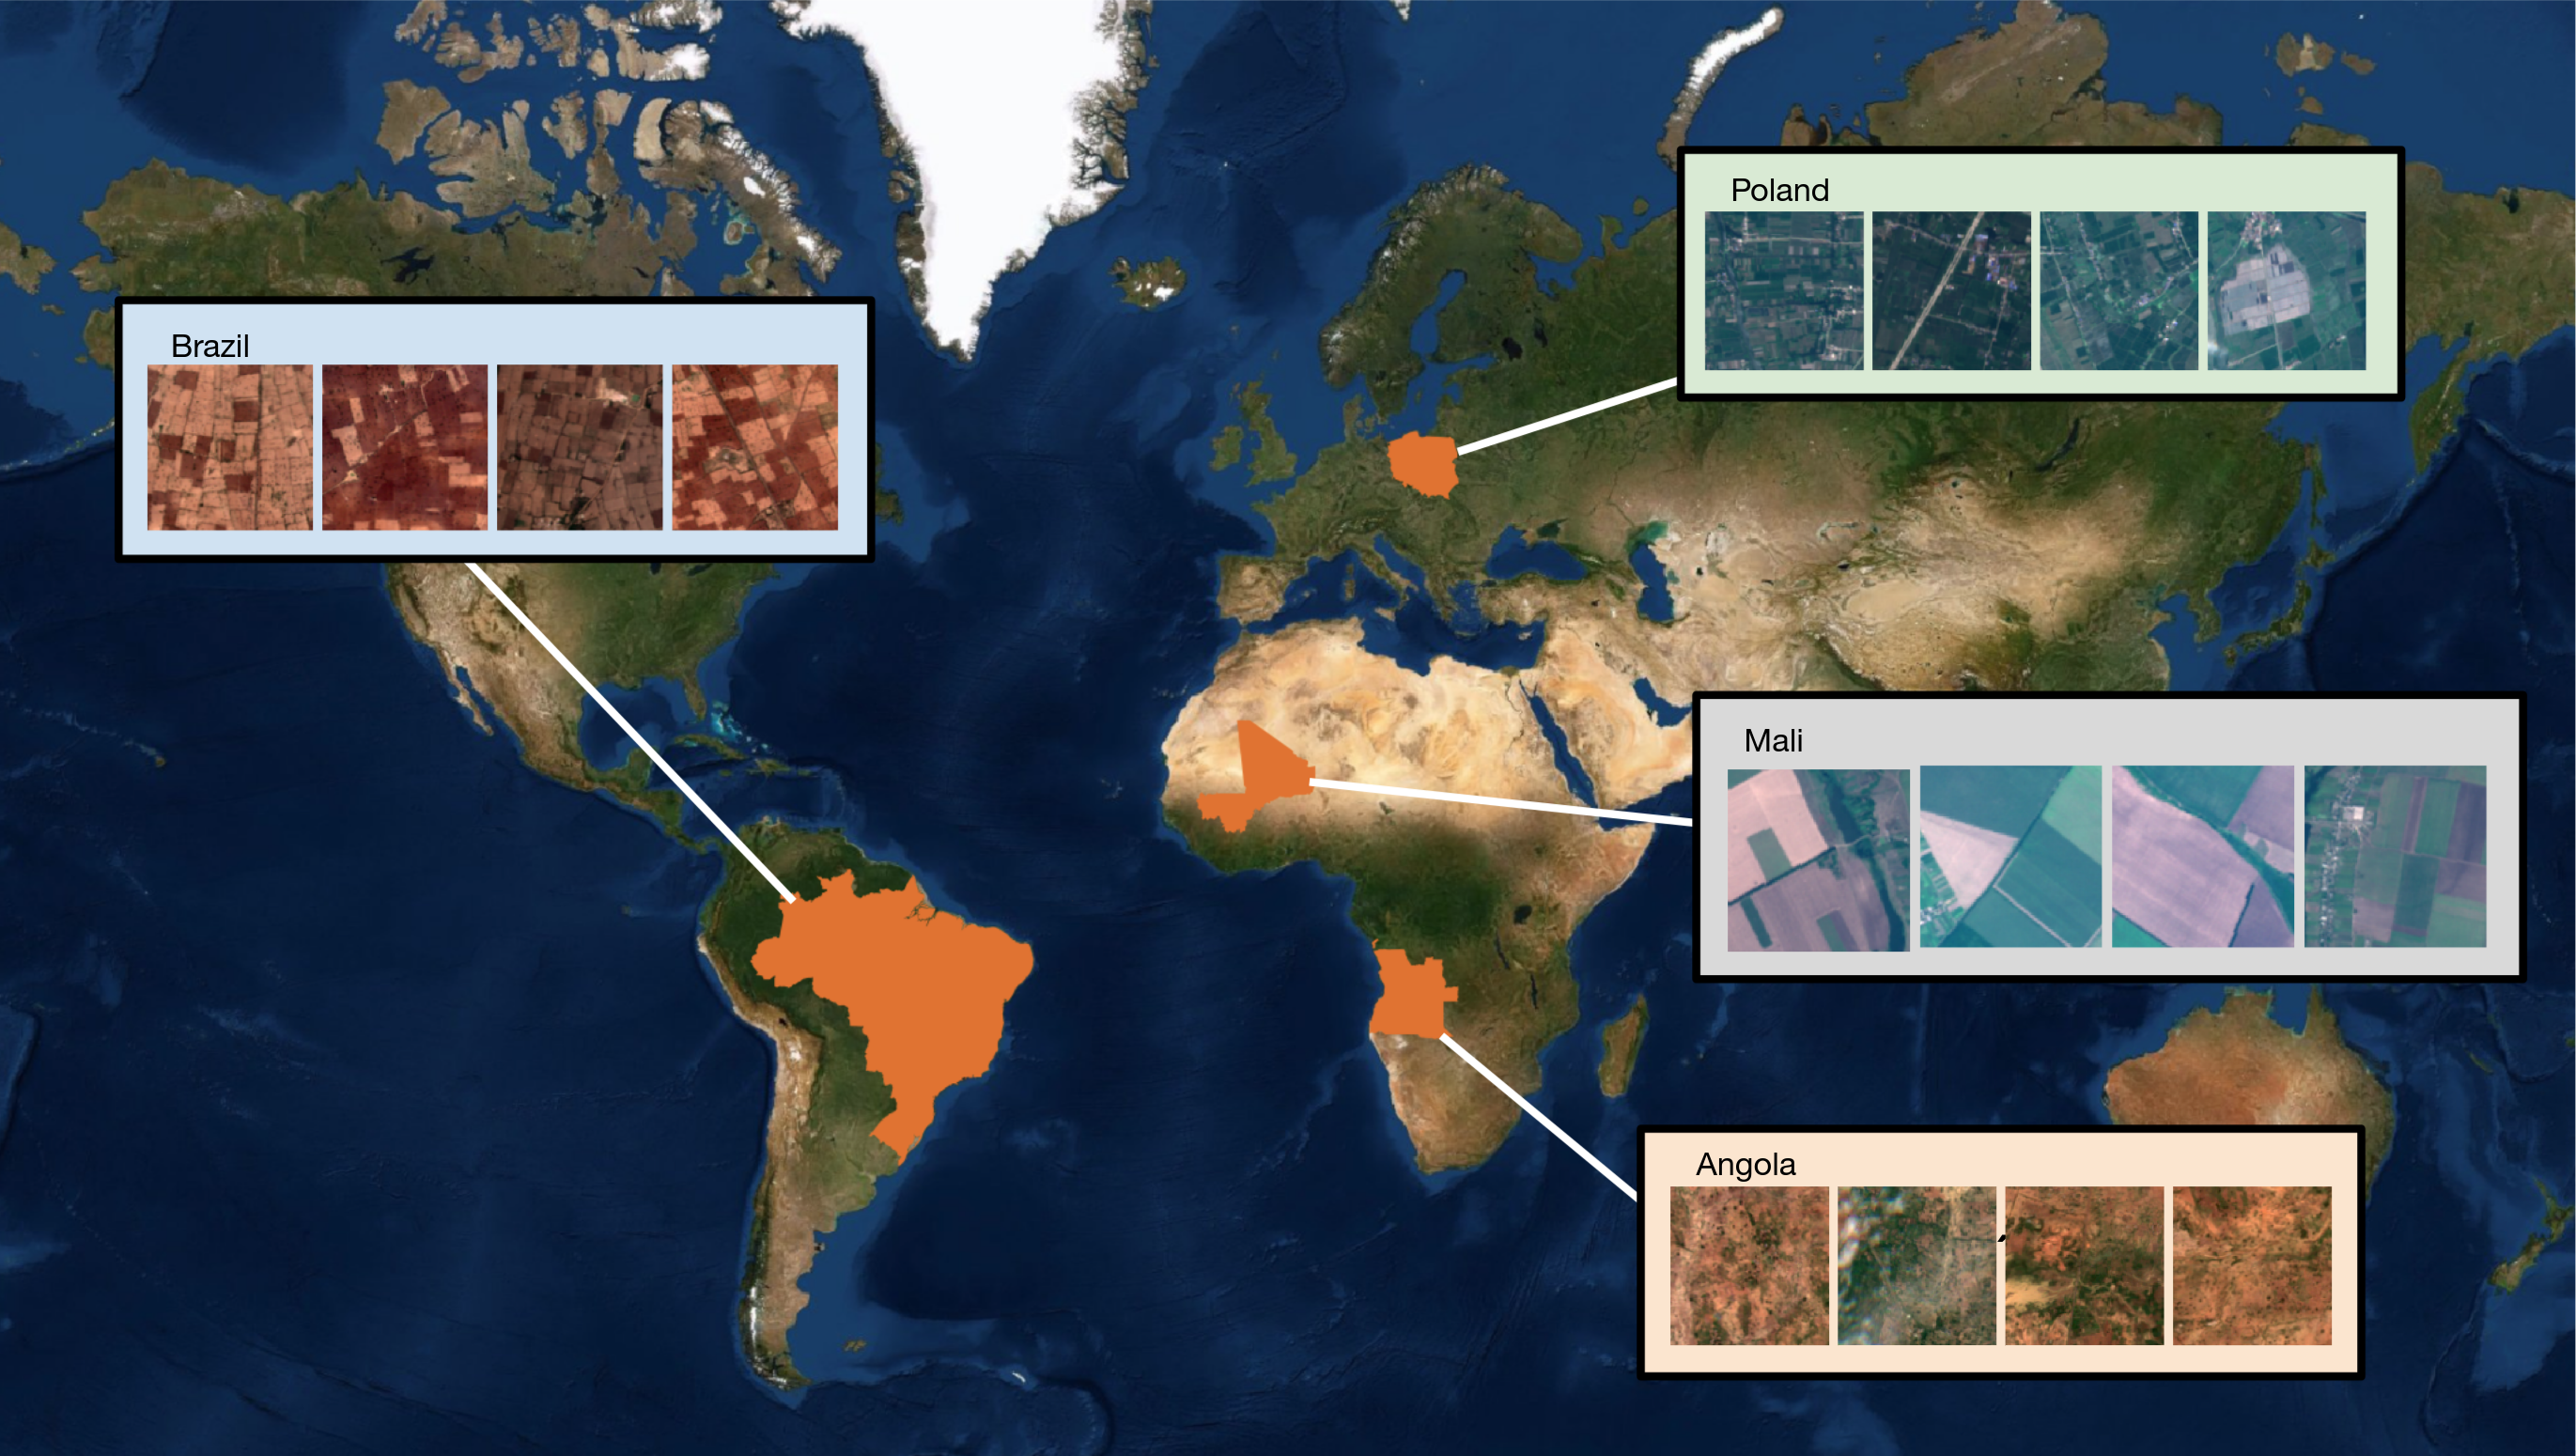
\includegraphics[width=\textwidth]{images/countries_globe}
		
		\vspace{0.5em}
		
		\scriptsize
		Figure from
		
		\citeapa{Rußwurm, M., Wang, S., Körner, M., \& Lobell, D. (2020). Meta-learning for few-shot land cover classification. In Proceedings of the ieee/cvf conference on computer vision and pattern recognition workshops (pp. 200-201).}
		
		\scriptsize
		Data from
		
		\citeapa{Schmitt, M., Hughes, L. H., Qiu, C., \& Zhu, X. X. (2019). SEN12MS--A Curated Dataset of Georeferenced Multi-Spectral Sentinel-1/2 Imagery for Deep Learning and Data Fusion. arXiv preprint arXiv:1906.07789.}
	\end{frame}
	
%	\begin{frame}{Domain and Task}
%		\begin{tikzpicture}
%		\node[label=domain](domain){$\mathcal{D} = \{\mathcal{X}, P(\mathcal{X})\}$};
%		\node[label=task, right=of domain](task){$\mathcal{T} = \{\mathcal{Y}, f(\cdot)\}$};
%		\end{tikzpicture}
%		\vfill\tiny
%		\citeapa{Pan, S. J., \& Yang, Q. (2009). A survey on transfer learning. IEEE Transactions on knowledge and data engineering, 22(10), 1345-1359.}
%		¨
%	\end{frame}

	\begin{frame}{Global Distribution Shift}
		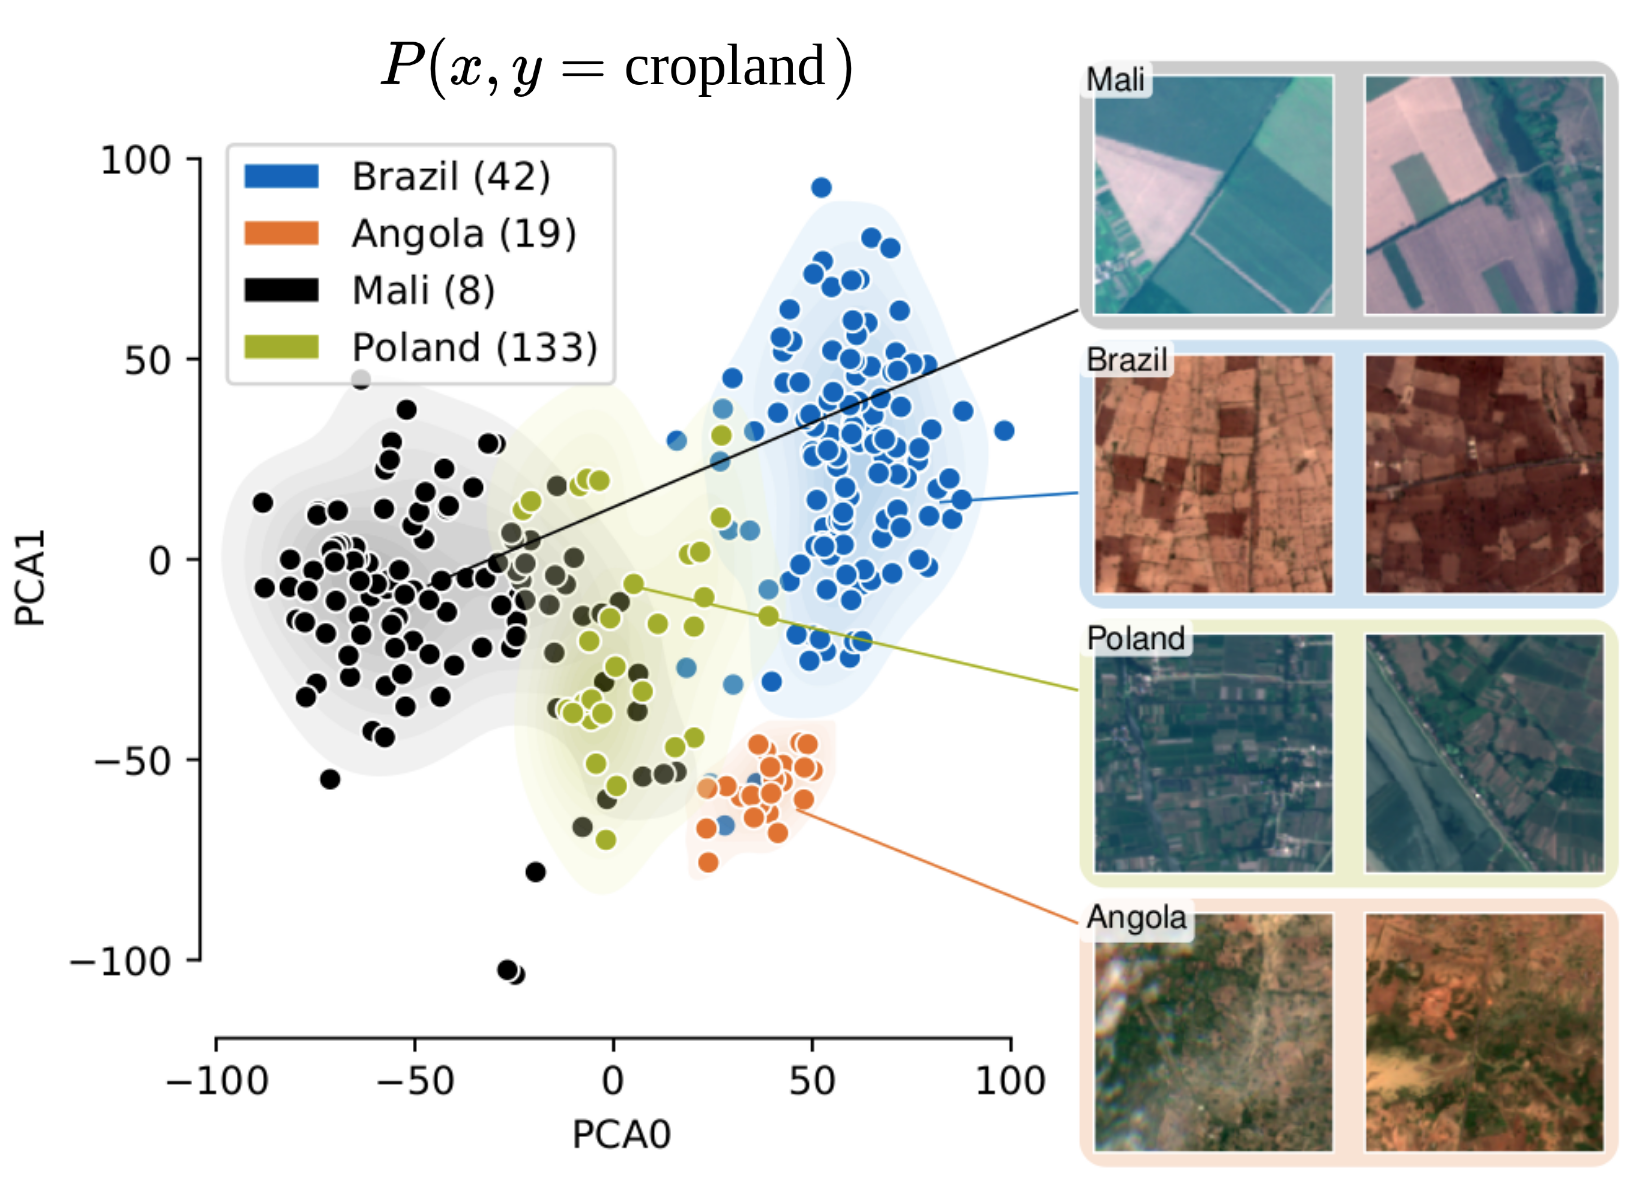
\includegraphics[width=.9\textwidth]{images/Sen12ms_distribution_shift}
		
		\scriptsize
		Figure from
		
		\citeapa{Rußwurm, M., Wang, S., Körner, M., \& Lobell, D. (2020). Meta-learning for few-shot land cover classification. In Proceedings of the ieee/cvf conference on computer vision and pattern recognition workshops (pp. 200-201).}
		
		\scriptsize
		Data from
		
		\citeapa{Schmitt, M., Hughes, L. H., Qiu, C., \& Zhu, X. X. (2019). SEN12MS--A Curated Dataset of Georeferenced Multi-Spectral Sentinel-1/2 Imagery for Deep Learning and Data Fusion. arXiv preprint arXiv:1906.07789.}
	\end{frame}
	
	\begin{frame}{Improve on the target Task/Domain}
		
		Option 1) Just train on target data "random initialization"
		
		\vspace{2em}
		
		\begin{tikzpicture}
		
		{\color{perle}
		\node(ds) at (0,0){$D \iidsim P(\mathcal{X} \times \mathcal{Y})$};
		\node at (-1,-1)(dstrain){$D_\text{train}$};
		\node at (1,-1)(dstest){$D_\text{test}$};
		
		\draw[-Stealth](ds) --node[midway, left=1em, font=\tiny, name=labelsplit]{random split} (dstrain);
		\draw[-Stealth](ds) -- (dstest);
		
		\node[draw, rounded corners, fit=(ds)(dstrain)(dstest)(labelsplit), label={above: Source Task/Domain\phantom{g}}]{};
		}
		
		\begin{scope}[xshift=5cm]
		\node(Q) at (0,0){$D \iidsim Q(\mathcal{X} \times \mathcal{Y})$};
		\node at (-1,-1)(dsqtrain){$D_\text{train}$};
		\node at (1,-1)(dsqtest){$D_\text{test}$};
		\end{scope}
		
		\node[below=of dsqtrain, label={[font=\tiny]left:train model}] (weightsq) {$f_\theta$};
		\draw[-Stealth] (dsqtrain) -- (weightsq);
		
		\draw[-Stealth](Q) --node[midway, left=0.5em, font=\tiny, name=labelqsplit]{random split} (dsqtrain);
		\draw[-Stealth](Q) -- (dsqtest);
		
		\node[draw, rounded corners, fit=(Q)(dsqtrain)(dsqtest)(labelqsplit), label={above: Target Task/Domain}]{};
		
		\node[below=of dsqtest] (oodloss) {$\mathcal{L}$};
%		\node[below=0em of oodloss, text width=3cm, font=\scriptsize](oodlabel){"out-of-domain" or \\ "out-of-distribution" \\ generalization};
%		
		\draw[-Stealth] (weightsq) -- node[midway,above,font=\tiny]{compare with $f_Q(\cdot)$} (oodloss);
		\draw[-Stealth] (dsqtest) -- (oodloss);
		
		\end{tikzpicture}
	\end{frame}

	\begin{frame}{Improve on the target Task/Domain}
		
		Option 2) "Pretrain" on Source finetune on Target 
		
		\vspace{2em}
		
		\begin{tikzpicture}
			\node(ds) at (0,0){$D \iidsim P(\mathcal{X} \times \mathcal{Y})$};
			\node at (-1,-1)(dstrain){$D_\text{train}$};
			\node at (1,-1)(dstest){$D_\text{test}$};
			
			\draw[-Stealth](ds) --node[midway, left=1em, font=\tiny, name=labelsplit]{random split} (dstrain);
			\draw[-Stealth](ds) -- (dstest);
			
			\node[draw, rounded corners, fit=(ds)(dstrain)(dstest)(labelsplit), label={above: Source Task/Domain\phantom{g}}]{};
			
			\node[below=of dstrain, label={[font=\tiny]left:train model}] (weights) {$f_\theta$};
			\draw[-Stealth] (dstrain) -- (weights);
			
%			\node[below=of dstest] (testloss) {$\mathcal{L}_\text{in}$};
			\draw[Stealth-] (dstest) -- node[midway, right, font=\tiny]{generalize in dist.} (weights);
			\draw[-Stealth] (weights) -- node[midway,above,font=\tiny]{initialize} (weightsq);
			
		\begin{scope}[xshift=5cm]
		\node(Q) at (0,0){$D \iidsim Q(\mathcal{X} \times \mathcal{Y})$};
		\node at (-1,-1)(dsqtrain){$D_\text{train}$};
		\node at (1,-1)(dsqtest){$D_\text{test}$};
		\end{scope}
		
		\node[below=of dsqtrain] (weightsq) {$f_\theta$};
		\draw[-Stealth] (dsqtrain) -- node[midway, left, font=\tiny]{finetune} (weightsq);
		
		\draw[-Stealth](Q) --node[midway, left=0.5em, font=\tiny, name=labelqsplit]{random split} (dsqtrain);
		\draw[-Stealth](Q) -- (dsqtest);
		
		\node[draw, rounded corners, fit=(Q)(dsqtrain)(dsqtest)(labelqsplit), label={above: Target Task/Domain}]{};
		
		\node[below=of dsqtest] (oodloss) {$\mathcal{L}$};
		%		\node[below=0em of oodloss, text width=3cm, font=\scriptsize](oodlabel){"out-of-domain" or \\ "out-of-distribution" \\ generalization};
		%		
		\draw[-Stealth] (weightsq) -- node[midway,above,font=\tiny]{compare with $f_Q(\cdot)$} (oodloss);
		\draw[-Stealth] (dsqtest) -- (oodloss);
		
		\end{tikzpicture}
		
		\vfill
		
		{	\scriptsize
			Side Note: "Transfer Learning aims to help improve the learning of the target predictive function $f_Q(\cdot)$ for the target domain using the knowledge in $\mathcal{D}_s$ and $\mathcal{T}_s$ where $\mathcal{D}_s \neq \mathcal{D}_t$ and $\mathcal{T}_s \neq \mathcal{T}_t$" \par
		}
		\vspace{.5em}
			\citeapa{Qiang Yang; Yu Zhang, Wenyuan Dai; Sinno Jialin Pan (Editors) (2020). Transfer learning. Cambridge University Press. DOI 9781139061773}
		
	\end{frame}

	\begin{frame}
		
	\end{frame}
	
	\begin{frame}{A Frame Title}
		
		\begin{columns}
			\column{.5\textwidth}
			
			
			This is the frame content
			\begin{itemize}
				\item with some itemize objects
				\item and another one
			\end{itemize}
			
			Enumerates should work too
			\begin{enumerate}
				\item one
				\item two
			\end{enumerate}
		
			\column{.5\textwidth}
			
			A second column with other content, maybe more text, or something \emph{emphasized}. For more, highlight in \emphred{red} or \emphblue{blue}.
			
			
			
		\end{columns}
		
	\end{frame}

		
		\begin{frame}<presentation:9,13,14,15>%1-9,
			\frametitle{Deep Neural Networks}
			\centering
			
			\newcommand{\V}[1]{\ensuremath{\mathsymbol{\lowercase{#1}}}}
\newcommand{\M}[1]{\ensuremath{\mathsymbol{\uppercase{#1}}}}
%
%\newcommand{\mathbf{w}}{\ensuremath{\M{W}}}
%\newcommand{\mathbf{w}}{\ensuremath{\M{W}}}
\newcommand{\VBias}{\ensuremath{\V{b}}}
\newcommand{\VInput}{\DataVec}
\newcommand{\VHidden}{\ensuremath{\V{h}}}
\newcommand{\FActivation}{\ensuremath{\sigma}}
\newcommand{\VCellState}{\ensuremath{\V{c}}}
\newcommand{\VForgetGate}{\ensuremath{\V{f}}}
\newcommand{\VModulationGate}{\ensuremath{\V{j}}}
\newcommand{\VInputGate}{\ensuremath{\V{i}}}
\newcommand{\VOutputGate}{\ensuremath{\V{o}}}


\tikzstyle{circ} = [circle, draw=white, fill=tumblue, inner sep=1pt]
\newcommand{\fcn}{
	\begin{tikzpicture}[scale=0.2, rotate=0, baseline=-.25em, inner sep=1pt]
	\node[circ](a0) at (0,-1){};
	\node[circ](a1) at (0,0){};
	\node[circ](a2) at (0,1){};
	
	\node[circ](b0) at (1,-0.5){};
	\node[circ](b1) at (1,0.5){};
	
	\draw[-] (a0) -- (b0);
	\draw[-] (a1) -- (b0);
	\draw[-] (a2) -- (b0);
	
	\draw[-] (a0) -- (b1);
	\draw[-] (a1) -- (b1);
	\draw[-] (a2) -- (b1);
	
	\end{tikzpicture}
}


\newcommand{\earth}{
	\begin{tikzpicture}[baseline=-.25em, inner sep=0]
	\node{
\includegraphics[width=8mm]{images/icons/earth}};
	\end{tikzpicture}
}

\newcommand{\sat}{
	\begin{tikzpicture}[baseline=-.25em, inner sep=0]
	\node[rotate=270,anchor=center]{
\includegraphics[width=8mm]{images/icons/sat2}};
	\end{tikzpicture}
}

\newcommand{\hidden}[1]{
	\begin{tikzpicture}[scale=.1, baseline=-.25em]	
	%\draw[step=1.0,black,thin] (0,0) grid (#1,1);
	\foreach \i in {1,...,#1}{
		\node[circle, draw=white, fill=tumbluelight, inner sep=1pt] at (\i,0){};
	}
	\end{tikzpicture}
}

\newcommand{\drawvector}[1]{
	\begin{tikzpicture}[scale=.1, baseline=-.25em]	
	%\draw[step=1.0,black,thin] (0,0) grid (#1,1);
	\foreach \i in {1,...,#1}{
		\node[circ] at (\i,0){};
	}
	\end{tikzpicture}
}
\tikzstyle{proba} = [circle, draw=tumgray, inner sep=2.5pt, fill=tumorange]
\newcommand{\drawprobas}[5]{
	\begin{tikzpicture}[scale=.3, baseline=-.25em]	
	
	\node[proba, fill=tumblue!#1] at (0,-2){};
	\node[proba, fill=tumblue!#2] at (0,-1){};
	\node[proba, fill=tumblue!#3] at (0,-0){};
	\node[proba, fill=tumblue!#4] at (0,1){};
	\node[proba, fill=tumblue!#5] at (0,2){};
	\end{tikzpicture}
}



\newcommand{\vegetationsmodell}{
	\begin{tikzpicture}[scale=0.5, rotate=0, baseline=-.25em, minimum width=0cm, minimum height=0cm]
	\node[proba](a0) at (0,-1){};
	\node[proba](a1) at (0,0){};
	\node[proba](a2) at (0,1){};
	
	\node[proba](b0) at (1,-0.5){};
	\node[proba](b1) at (1,0.5){};
	
	\draw[-] (a0) -- (b0);
	\draw[-] (a1) -- (b0);
	\draw[-] (a2) -- (b0);
	
	\draw[-] (a0) -- (b1);
	\draw[-] (a1) -- (b1);
	\draw[-] (a2) -- (b1);
	
	%	\node[fit=(a0)(a2)(b1)](node name){};
	
	\end{tikzpicture}
}

\tikzstyle{tsmark} = [mark=|,mark size=2pt]

\colorlet{tumgray}{gray}
\colorlet{tumorange}{carotte}
\colorlet{tumblue}{leman}
\colorlet{tumbluedark}{canard}


\begin{tikzpicture}[node distance=.1em]
			\node[minimum width=1cm, minimum height=1.5cm, draw,rounded corners](veg) at (0,0){\vegetationsmodell};
			\coordinate[below=1em of veg](labelreference);
			\node(annotveg) at (labelreference){$f_{{\mathbf{w}}}$};
			\visible<1>{
				\node[above=2em of veg, font=\small, xshift=4em, text width=17em](annotf){\textbf{{\Large \color{tumblue}differentiable} non-linear function} \\ width randomly initialized weights $\mathbf{w}$};
				\draw[-stealth] (annotf) -- (veg);
			}
			\node[right=1em of veg, inner sep=0](input){%
				%		$\left(
				\only<1-12>{%
					$\mathbf{X}$%\rawtimeseriestwo{12-71456800.csv}%
				}%
				\only<0>{%9-12
					\begin{tikzpicture}[baseline=-1.5em, xscale=0.3, yscale=-.3]
					\foreach \x in {0,...,15}{
						\node[draw=tumgraylight, circle, fill=b2color, text=white, text opacity=1, font=\small, inner sep=2.5pt](d) at (\x,0){};
						\node[draw=tumgraylight, circle, fill=b3color, text=white, text opacity=1, font=\small, inner sep=2.5pt](d) at (\x,1){};
						\node[draw=tumgraylight, circle, fill=b4color, text=white, text opacity=1, font=\small, inner sep=2.5pt](d) at (\x,2){};
						\node[draw=tumgraylight, circle, fill=b5color, text=white, text opacity=1, font=\small, inner sep=2.5pt](d) at (\x,3){};
						\node[draw=tumgraylight, circle, fill=b6color, text=white, text opacity=1, font=\small, inner sep=2.5pt](d) at (\x,4){};
					}
					\end{tikzpicture}%
				}%
				\only<13-14>{
					\begin{tikzpicture}
					\node[draw, rounded corners, minimum width=1cm, minimum height=1.5cm](preproc){
\includegraphics[width=.8cm]{images/icons/gears}};
					\node[right=1.5em of preproc](input){$\mathbf{X}$};%\rawtimeseriestwo{12-71456800_raw.csv}
					\node[font=\huge,left=0em of input, inner sep=0](bopen){$\Bigg($};
					\node[font=\huge, right=0em of input, inner sep=0](bopen){$\Bigg)$};
					\end{tikzpicture}
				}
				\only<15>{
					$\mathbf{X}$%\rawtimeseriestwo{12-71456800_raw.csv}
				}
			};% \rawtimeseries{prep77770412.csv}
			\only<13,14>{
				\node[right=1.5em of annotveg]{$f_{{\mathbf{w}}_\text{preproc}}$};
			}
			
			
			\node(annotinput) at (labelreference -| input){$\mathbf{X}$};
			\node[font=\huge,left=0em of input, inner sep=0](bopen){$\Bigg($};
			\node[font=\huge, right=0em of input, inner sep=0](bopen){$\Bigg)$};
			\node[left= of veg, font=\huge](equals){$=$};
			\only<-5>{\node[left= of equals](probas){\drawprobas{10}{30}{10}{20}{10}};}
			\visible<5>{\node[left= of equals](probas){\drawprobas{20}{30}{50}{20}{30}};}
			\visible<6>{\node[left= of equals](probas){\drawprobas{30}{40}{30}{50}{20}};}
			\visible<7>{\node[left= of equals](probas){\drawprobas{20}{20}{20}{80}{10}};}
			\visible<8->{\node[left= of equals](probas){\drawprobas{10}{30}{10}{100}{10}};}
			\node(annotprobas) at (labelreference -| probas){$\hat{y}$};
			\visible<2->{
				\node[left= 5em of probas](gt){\drawprobas{0}{0}{0}{100}{0}};
				\node(annotgt) at (labelreference -| gt){$\mathbf{y}$};
			}
			\visible<3->{
				\draw[stealth-stealth] (gt) -- node[midway,above](loss){$\mathcal{L}(\mathbf{y},\hat{y})$} (probas);
			}
			
			
			\visible<4->{\draw[-stealth] (loss)  to [out=60,in=135,looseness=1] node[midway,above]{${\mathbf{w}} \leftarrow \mathbf{w} - \frac{\partial \mathcal{L}}{\partial {\mathbf{w}}}$} (veg);}
			
			
			\only<9-12>{
				\node[above=10em of annotinput, font=\Large\bfseries, text=white, fill=tumbluedark, rounded corners](e1){End};
				\node[above=10em of annotgt, font=\Large\bfseries, text=white, fill=tumbluedark, rounded corners](e2){End};
				\node[above=10em of annotveg, text=white, fill=tumbluedark, font=\Large\bfseries, rounded corners](to){to};
				\draw[thick, tumbluedark] (e1) -- (to) -- (e2);
			}
			
			\only<10>{
				\node[below=of annotinput]{Satellite Time Series};
				\node[below=of annotgt]{Crop Types};
			}
			
			\only<11>{
				\node[below=of annotinput]{Images (single Band)};
				\node[below=of annotgt]{Cats and Dogs};
			}
			\only<12>{
				\node[below=of annotinput]{Text and Language};
				\node[below=of annotgt]{Sentiment};
			}
			
			\only<14>{
				\coordinate(fpreproc) at ($ (veg)+(3.5em,0) $);
				
				\draw[-stealth, dotted, red, thick] (loss)  to [out=-60,in=-135,looseness=1] node[midway,below]{\xcancel{$\frac{\partial \mathcal{L}}{\partial {\mathbf{w}}_\text{preproc}}$}} ($ (fpreproc)+(0,-2.3em) $);
				
				\node[above right=6em of fpreproc](a){$\mathbf{w}_\text{sel}$: start/end of vegetation period};
				\node[below right=6em of fpreproc](b){$\mathbf{w}_\text{atm}$: atmospheric parameters};
				\node[below right=7em and 2em of fpreproc, text width=14em](c){$\mathbf{w}_\text{cl}$: cloud classifier trained on different training set};
				\draw[-stealth, shorten >=4em] (a.south west) -- (fpreproc);
				\draw[-stealth, shorten >=4em] (b.north west) -- (fpreproc);
				\draw[-stealth, shorten >=4em] (c.north west) -- (fpreproc);
			}
			
		\end{tikzpicture}
	\end{frame}

	\begin{frame}{Colors}
		\centering
		\begin{tikzpicture}[xscale=2.6, yscale=-2]
		\tikzstyle{colorbox} = [minimum width=1.8cm, minimum height=1.8cm, text width=1.5cm, font=\scriptsize]
		
		\node(rouge) at (0,0)[fill=rouge,text=white, colorbox]{rouge};
		\node(leman) at (0,1)[fill=leman,text=white, colorbox]{leman};
		\node(grosseille) at (0,2)[fill=grosseille,text=white, colorbox]{grosseille};
		\node(canard) at (0,3)[fill=canard,text=white, colorbox]{canard};
		\node(montrose) at (1,0)[fill=montrose,text=white, colorbox]{montrose};
		\node(perle) at (1,1)[fill=perle,text=white, colorbox]{perle};
		\node(vertedeau) at (1,2)[fill=vertedeau,text=white, colorbox]{vertedeau};
		\node(rose) at (1,3)[fill=rose,text=white, colorbox]{rose};
		\node(acier) at (2,0)[fill=acier,text=white, colorbox]{acier};
		\node(soufre) at (2,1)[fill=soufre,text=white, colorbox]{soufre};
		\node(carotte) at (2,2)[fill=carotte,text=white, colorbox]{carotte};
		\node(zinzolin) at (2,3)[fill=zinzolin,text=white, colorbox]{zinzolin};
		\node(chartreuse) at (3,0)[fill=chartreuse,text=white, colorbox]{chartreuse};
		\node(marron) at (3,1)[fill=marron,text=white, colorbox]{marron};
		\node(ardoise) at (3,2)[fill=ardoise,text=white, colorbox]{ardoise};
		\node(taupe) at (3,3)[fill=taupe,text=white, colorbox]{taupe};
		
		\end{tikzpicture}
		
		
\end{frame}

\end{document}